\documentclass[8pt,aspectratio=169]{beamer}
\usetheme{Madrid}
\usepackage{graphicx,booktabs,adjustbox,multicol,amsmath,amssymb,listings,xcolor,colortbl,multirow}
\definecolor{mlblue}{RGB}{0,102,204}
\definecolor{mlpurple}{RGB}{51,51,178}
\definecolor{mllavender}{RGB}{173,173,224}
\definecolor{mllavender2}{RGB}{193,193,232}
\definecolor{mllavender3}{RGB}{204,204,235}
\definecolor{mllavender4}{RGB}{214,214,239}
\definecolor{mlorange}{RGB}{255,127,14}
\definecolor{mlgreen}{RGB}{44,160,44}
\definecolor{mlred}{RGB}{214,39,40}
\definecolor{mlgray}{RGB}{127,127,127}
% Solidity colors
\definecolor{solkeyword}{RGB}{0,102,153}
\definecolor{solstring}{RGB}{163,21,21}
\definecolor{solcomment}{RGB}{0,128,0}
\definecolor{solnumber}{RGB}{0,128,128}
\setbeamercolor{palette primary}{bg=mllavender3,fg=mlpurple}
\setbeamercolor{palette secondary}{bg=mllavender2,fg=mlpurple}
\setbeamercolor{palette tertiary}{bg=mllavender,fg=white}
\setbeamercolor{palette quaternary}{bg=mlpurple,fg=white}
\setbeamercolor{structure}{fg=mlpurple}
\setbeamercolor{title}{fg=mlpurple}
\setbeamercolor{frametitle}{fg=mlpurple,bg=mllavender3}
\setbeamercolor{block title}{bg=mllavender2,fg=mlpurple}
\setbeamercolor{block body}{bg=mllavender4,fg=black}
\setbeamertemplate{navigation symbols}{}
\setbeamertemplate{itemize items}[circle]
\setbeamersize{text margin left=5mm,text margin right=5mm}
\newcommand{\bottomnote}[1]{\vfill\vspace{-2mm}\textcolor{mllavender2}{\rule{\textwidth}{0.4pt}}\vspace{1mm}\footnotesize\textbf{#1}}
% Solidity language definition
\lstdefinelanguage{Solidity}{
  keywords={pragma, solidity, contract, function, public, private, external, internal, view, pure, payable, returns, return, if, else, for, while, mapping, address, uint, uint256, int, string, bool, bytes, bytes32, event, emit, modifier, require, constructor, memory, storage, calldata, msg, sender, value, this, new, delete, true, false, import, is, constant, override, virtual, interface, library, abstract, struct, enum, unchecked, assembly, abi, encode, decode, keccak256, receive, fallback},
  keywordstyle=\color{solkeyword}\bfseries,
  sensitive=true,
  comment=[l]{//},
  morecomment=[s]{/*}{*/},
  commentstyle=\color{solcomment}\ttfamily,
  stringstyle=\color{solstring}\ttfamily,
  morestring=[b]',
  morestring=[b]"
}
\lstset{language=Solidity,basicstyle=\ttfamily\scriptsize,breaklines=true,frame=single,backgroundcolor=\color{mllavender4},numbers=left,numberstyle=\tiny\color{mlgray},numbersep=5pt,tabsize=2,showstringspaces=false}
\usepackage{tikz,pgfplots}
\pgfplotsset{compat=1.18}
\usetikzlibrary{arrows.meta,positioning,shapes.geometric,calc,chains,decorations.pathmorphing,automata,fit}
\title{Privacy \& Zero-Knowledge Proofs: From Theory to Application}
\subtitle{Standalone Technical Lecture}
\author{Prof.~Dr.~Joerg Osterrieder}
\institute{University Lecture Series}
\date{\today}

\begin{document}

%% ============================================================
%% OPENING FRAMES
%% ============================================================

% Frame 1: Title
\begin{frame}
\titlepage
\end{frame}

% Frame 2: Lecture Roadmap
\begin{frame}{Lecture Roadmap}
\begin{columns}[T]
\column{0.55\textwidth}
\vspace{2mm}
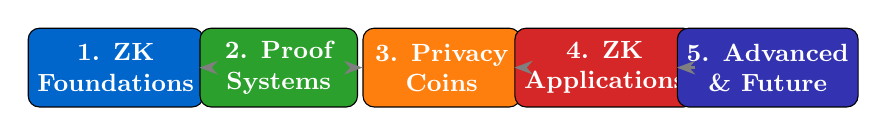
\begin{tikzpicture}[scale=0.9]
  \node[draw,fill=mlblue,text=white,rounded corners=4pt,
        minimum width=2.0cm,minimum height=1.0cm,align=center,font=\small\bfseries]
        (b1) at (0,0) {1. ZK\\Foundations};
  \node[draw,fill=mlgreen,text=white,rounded corners=4pt,
        minimum width=2.0cm,minimum height=1.0cm,align=center,font=\small\bfseries]
        (b2) at (2.3,0) {2. Proof\\Systems};
  \node[draw,fill=mlorange,text=white,rounded corners=4pt,
        minimum width=2.0cm,minimum height=1.0cm,align=center,font=\small\bfseries]
        (b3) at (4.6,0) {3. Privacy\\Coins};
  \node[draw,fill=mlred,text=white,rounded corners=4pt,
        minimum width=2.0cm,minimum height=1.0cm,align=center,font=\small\bfseries]
        (b4) at (6.9,0) {4. ZK\\Applications};
  \node[draw,fill=mlpurple,text=white,rounded corners=4pt,
        minimum width=2.0cm,minimum height=1.0cm,align=center,font=\small\bfseries]
        (b5) at (9.2,0) {5. Advanced\\\& Future};
  \draw[-{Stealth},thick,mlgray] (b1.east) -- (b2.west);
  \draw[-{Stealth},thick,mlgray] (b2.east) -- (b3.west);
  \draw[-{Stealth},thick,mlgray] (b3.east) -- (b4.west);
  \draw[-{Stealth},thick,mlgray] (b4.east) -- (b5.west);
\end{tikzpicture}
\vspace{3mm}

\column{0.45\textwidth}
\begin{block}{Learning Objectives}
\footnotesize
\begin{itemize}
  \item Formalise ZK proof definitions and properties
  \item Compare SNARK, STARK, and Bulletproof systems
  \item Analyse privacy coin cryptography (Monero, Zcash)
  \item Evaluate ZK-rollup architectures and zkEVM types
  \item Assess future directions in ZK technology
\end{itemize}
\end{block}
\vspace{1mm}
\begin{block}{Prerequisites}
\footnotesize
\begin{itemize}
  \item Lessons 1--5: Blockchain fundamentals, smart contracts, DeFi
  \item L12 Tokenomics recommended for economic context
\end{itemize}
\end{block}
\end{columns}
\bottomnote{Duration: 90 minutes | 5 sections | \textasciitilde55 frames | Prerequisite: Lessons 1--5}
\end{frame}

% Frame 3: Table of Contents
\begin{frame}{Table of Contents}
\tableofcontents
\bottomnote{Navigate through 5 sections from ZK foundations to advanced topics and future directions}
\end{frame}

\begin{frame}{Learning Objectives}
By the end of this lecture, you will be able to:
\begin{enumerate}
\item \textbf{Explain} the formal definition of zero-knowledge proofs and the simulation paradigm
\item \textbf{Compare} proof systems (Groth16, PLONK, STARKs, Bulletproofs) on setup, size, and speed
\item \textbf{Analyze} privacy coin mechanisms (ring signatures, stealth addresses, shielded pools)
\item \textbf{Evaluate} ZK applications (rollups, identity, voting, confidential DeFi, zkML)
\item \textbf{Assess} hardware acceleration and post-quantum considerations for ZK systems
\end{enumerate}
\bottomnote{Bloom's taxonomy levels: Remember $\rightarrow$ Understand $\rightarrow$ Apply $\rightarrow$ Analyze $\rightarrow$ Evaluate $\rightarrow$ Create}
\end{frame}

%% ============================================================
%% SECTION 1: ZK PROOF FOUNDATIONS & MATHEMATICAL BASICS
%% ============================================================
\section{ZK Proof Foundations \& Mathematical Basics}

% Frame 4: Historical Context
\begin{frame}{Historical Context: The GMR Paper (1985)}
\begin{columns}[T]
\column{0.55\textwidth}
\begin{block}{The Breakthrough}
\footnotesize
Goldwasser, Micali, and Rackoff (1985) posed a revolutionary question:
\vspace{2mm}
\textit{``Can we prove a statement is true without revealing \textbf{why} it is true?''}
\vspace{2mm}
Their paper ``The Knowledge Complexity of Interactive Proof Systems'' introduced the concept of \textbf{zero-knowledge proofs}.
\end{block}
\vspace{2mm}
\begin{exampleblock}{\footnotesize Impact}
\footnotesize
This work earned the 2012 Turing Award and laid the foundation for all modern ZK systems used in blockchain today.
\end{exampleblock}

\column{0.45\textwidth}
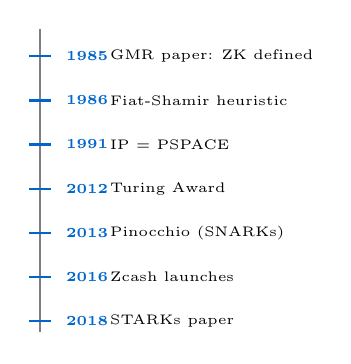
\begin{tikzpicture}[scale=0.7]
  \draw[thick,mlgray] (0,0) -- (0,5.5);
  \foreach \y/\yr/\evt in {
    5.0/1985/{GMR paper: ZK defined},
    4.2/1986/{Fiat-Shamir heuristic},
    3.4/1991/{IP = PSPACE},
    2.6/2012/{Turing Award},
    1.8/2013/{Pinocchio (SNARKs)},
    1.0/2016/{Zcash launches},
    0.2/2018/{STARKs paper}} {
    \draw[thick,mlblue] (-0.2,\y) -- (0.2,\y);
    \node[right,font=\tiny\bfseries,mlblue] at (0.3,\y) {\yr};
    \node[right,font=\tiny] at (1.1,\y) {\evt};
  }
\end{tikzpicture}
\end{columns}
\bottomnote{Goldwasser, Micali \& Rackoff showed that proof is about more than truth -- it's about knowledge transfer}
\end{frame}

% Frame 5: Formal Definition
\begin{frame}{Formal Definition of Zero-Knowledge Proofs}
\begin{columns}[T]
\column{0.55\textwidth}
\begin{block}{Interactive Proof System $(P, V)$}
\footnotesize
For a language $L \in \mathrm{NP}$ with witness relation $R$:
\end{block}
\vspace{1mm}
\begin{block}{1. Completeness}
\footnotesize
If $x \in L$ and the prover $P$ has a valid witness $w$:
\[
\Pr[V \text{ accepts} \mid (x,w) \in R] \geq 1 - \varepsilon
\]
An honest prover always convinces the verifier.
\end{block}
\vspace{1mm}
\begin{block}{2. Soundness}
\footnotesize
If $x \notin L$, for \textit{any} cheating prover $P^*$:
\[
\Pr[V \text{ accepts} \mid P^*] \leq \varepsilon
\]
No cheating prover can convince the verifier.
\end{block}

\column{0.45\textwidth}
\begin{block}{3. Zero-Knowledge}
\footnotesize
There exists a \textbf{simulator} $S$ such that:
\[
\text{View}_V(P(x,w)) \approx S(x)
\]
The verifier's ``view'' of the real interaction is \textit{computationally indistinguishable} from a simulation that doesn't know $w$.
\end{block}
\vspace{2mm}
\begin{alertblock}{\footnotesize Key Insight}
\footnotesize
The simulator produces fake transcripts that look identical to real ones. If the verifier can't tell the difference, it learned \textbf{nothing} from the real interaction.
\end{alertblock}
\end{columns}
\bottomnote{The three properties -- completeness, soundness, zero-knowledge -- form the foundation of all ZK systems}
\end{frame}

% Frame 6: The Simulation Paradigm
\begin{frame}{The Simulation Paradigm}
\begin{columns}[T]
\column{0.5\textwidth}
\begin{block}{Real World}
\footnotesize
\begin{center}
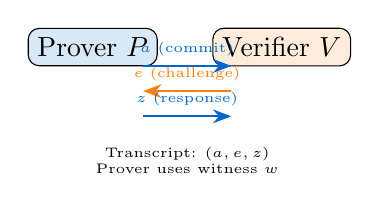
\begin{tikzpicture}[scale=0.8]
  \node[draw,fill=mlblue!15,rounded corners,minimum width=1.5cm] (P) at (0,2) {Prover $P$};
  \node[draw,fill=mlorange!15,rounded corners,minimum width=1.5cm] (V) at (3,2) {Verifier $V$};
  \draw[-{Stealth},mlblue,thick] (0.8,1.7) -- (2.2,1.7) node[midway,above,font=\tiny] {$a$ (commit)};
  \draw[-{Stealth},mlorange,thick] (2.2,1.3) -- (0.8,1.3) node[midway,above,font=\tiny] {$e$ (challenge)};
  \draw[-{Stealth},mlblue,thick] (0.8,0.9) -- (2.2,0.9) node[midway,above,font=\tiny] {$z$ (response)};
  \node[font=\tiny,align=center] at (1.5,0.2) {Transcript: $(a, e, z)$\\Prover uses witness $w$};
\end{tikzpicture}
\end{center}
\end{block}

\column{0.5\textwidth}
\begin{block}{Simulated World}
\footnotesize
\begin{center}
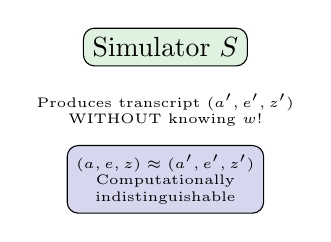
\begin{tikzpicture}[scale=0.8]
  \node[draw,fill=mlgreen!15,rounded corners,minimum width=2cm] (S) at (1.5,2) {Simulator $S$};
  \node[font=\tiny,align=center] at (1.5,1.0) {Produces transcript $(a', e', z')$\\WITHOUT knowing $w$!};
  \node[draw,fill=mllavender4,rounded corners,font=\tiny,align=center] at (1.5,-0.1) {$(a, e, z) \approx (a', e', z')$\\Computationally\\indistinguishable};
\end{tikzpicture}
\end{center}
\end{block}
\end{columns}
\vspace{2mm}
\begin{columns}[T]
\column{0.33\textwidth}
\begin{block}{\centering Perfect ZK}
\footnotesize
Distributions are \textbf{identical}. Information-theoretically secure.
\end{block}
\column{0.33\textwidth}
\begin{block}{\centering Statistical ZK}
\footnotesize
Distributions are \textbf{statistically close}. Negligible difference.
\end{block}
\column{0.33\textwidth}
\begin{block}{\centering Computational ZK}
\footnotesize
No PPT algorithm can \textbf{distinguish} them. Relies on hardness.
\end{block}
\end{columns}
\bottomnote{The simulation paradigm is the gold standard for proving zero-knowledge -- if it can be simulated, nothing was learned}
\end{frame}

% Frame 7: Commitment Schemes
\begin{frame}{Commitment Schemes}
\begin{columns}[T]
\column{0.5\textwidth}
\begin{block}{Pedersen Commitment}
\footnotesize
Let $\mathbb{G}$ be a group of prime order $q$ with generators $g, h$:
\[
C = g^v \cdot h^r
\]
where $v$ is the committed value and $r \stackrel{\$}{\leftarrow} \mathbb{Z}_q$ is randomness.
\end{block}
\vspace{1mm}
\begin{block}{Properties}
\footnotesize
\begin{itemize}
  \item \textbf{Perfectly Hiding:} For any $v$, the commitment $C$ is uniformly distributed (information-theoretic)
  \item \textbf{Computationally Binding:} Opening to a different value requires solving DLog (breaking $\log_g h$)
\end{itemize}
\end{block}
\vspace{1mm}
\begin{exampleblock}{\footnotesize Homomorphic Property}
\footnotesize
\[
C(v_1, r_1) \cdot C(v_2, r_2) = C(v_1 + v_2, r_1 + r_2)
\]
Enables arithmetic on committed values!
\end{exampleblock}

\column{0.5\textwidth}
\footnotesize
\begin{tabular}{lcc}
\toprule
\textbf{Scheme} & \textbf{Hiding} & \textbf{Binding} \\
\midrule
Pedersen & Perfect & Computational \\
Hash-based & Computational & Perfect \\
ElGamal & Perfect & Computational \\
\bottomrule
\end{tabular}
\vspace{3mm}
\begin{alertblock}{\footnotesize Impossibility Result}
\footnotesize
A commitment scheme cannot be both \textit{perfectly hiding} and \textit{perfectly binding} simultaneously. One property must rely on computational assumptions.
\end{alertblock}
\vspace{2mm}
\begin{block}{Vector Pedersen Commitment}
\footnotesize
For vector $\vec{v} = (v_1, \ldots, v_n)$:
\[
C = h^r \cdot \prod_{i=1}^{n} g_i^{v_i}
\]
Commits to $n$ values in a single group element.
\end{block}
\end{columns}
\bottomnote{Pedersen commitments are the building block of Bulletproofs, Monero's RingCT, and many ZK systems}
\end{frame}

% Frame 8: Schnorr's Sigma Protocol
\begin{frame}{Sigma Protocols: Schnorr's Protocol}
\begin{columns}[T]
\column{0.55\textwidth}
\begin{block}{Goal}
\footnotesize
Prove knowledge of discrete logarithm $x$ such that $y = g^x$ without revealing $x$.
\end{block}
\vspace{1mm}
\begin{center}
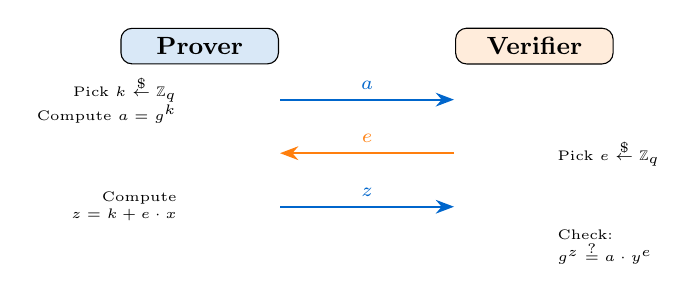
\begin{tikzpicture}[scale=0.85]
  \node[draw,fill=mlblue!15,rounded corners,minimum width=2cm,font=\small\bfseries] (P) at (0,3) {Prover};
  \node[draw,fill=mlorange!15,rounded corners,minimum width=2cm,font=\small\bfseries] (V) at (5,3) {Verifier};
  % Step 1
  \node[left,font=\tiny,align=right] at (-0.2,2.2) {Pick $k \stackrel{\$}{\leftarrow} \mathbb{Z}_q$\\Compute $a = g^k$};
  \draw[-{Stealth},mlblue,thick] (1.2,2.2) -- (3.8,2.2) node[midway,above,font=\scriptsize] {$a$};
  % Step 2
  \node[right,font=\tiny,align=left] at (5.2,1.4) {Pick $e \stackrel{\$}{\leftarrow} \mathbb{Z}_q$};
  \draw[-{Stealth},mlorange,thick] (3.8,1.4) -- (1.2,1.4) node[midway,above,font=\scriptsize] {$e$};
  % Step 3
  \node[left,font=\tiny,align=right] at (-0.2,0.6) {Compute\\$z = k + e \cdot x$};
  \draw[-{Stealth},mlblue,thick] (1.2,0.6) -- (3.8,0.6) node[midway,above,font=\scriptsize] {$z$};
  % Verification
  \node[right,font=\tiny,align=left] at (5.2,0.0) {Check:\\$g^z \stackrel{?}{=} a \cdot y^e$};
\end{tikzpicture}
\end{center}

\column{0.45\textwidth}
\begin{block}{Verification Equation}
\footnotesize
\[
g^z = g^{k + ex} = g^k \cdot g^{ex} = a \cdot (g^x)^e = a \cdot y^e
\]
\end{block}
\vspace{1mm}
\begin{block}{Properties}
\footnotesize
\begin{itemize}
  \item \textbf{Complete:} Honest prover always passes
  \item \textbf{Special Sound:} Two valid transcripts with same $a$ but different $e$ yield $x$
  \item \textbf{SHVZK:} Special Honest-Verifier ZK via simulation
\end{itemize}
\end{block}
\vspace{1mm}
\begin{exampleblock}{\footnotesize Fiat-Shamir Transform}
\footnotesize
Replace verifier's random $e$ with $e = H(a \| m)$:
\[
\text{Interactive} \xrightarrow{\text{Fiat-Shamir}} \text{Non-Interactive}
\]
This is how digital signatures (EdDSA) work!
\end{exampleblock}
\end{columns}
\bottomnote{Schnorr's protocol is the simplest sigma protocol -- it underlies EdDSA signatures and many ZK constructions}
\end{frame}

% Frame 9: KZG Polynomial Commitments
\begin{frame}{Polynomial Commitments (KZG)}
\begin{columns}[T]
\column{0.55\textwidth}
\begin{block}{Kate-Zaverucha-Goldberg Scheme}
\footnotesize
Commit to polynomial $p(x) = \sum_{i=0}^{d} c_i x^i$ using elliptic curve pairings.
\end{block}
\vspace{1mm}
\begin{block}{Setup (Trusted)}
\footnotesize
Secret $s \in \mathbb{F}_p$, publish structured reference string:
\[
\text{SRS} = \{[1]_1, [s]_1, [s^2]_1, \ldots, [s^d]_1, [1]_2, [s]_2\}
\]
where $[x]_1 = x \cdot G_1$ (group $\mathbb{G}_1$ element).
\end{block}
\vspace{1mm}
\begin{block}{Commitment}
\footnotesize
\[
C = [p(s)]_1 = \sum_{i=0}^{d} c_i \cdot [s^i]_1
\]
A single group element commits to the entire polynomial.
\end{block}

\column{0.45\textwidth}
\begin{block}{Evaluation Proof}
\footnotesize
To prove $p(z) = v$, compute quotient:
\[
q(x) = \frac{p(x) - v}{x - z}
\]
Proof: $\pi = [q(s)]_1$
\end{block}
\vspace{1mm}
\begin{block}{Verification (Pairing Check)}
\footnotesize
\[
e(C - [v]_1,\ [1]_2) \stackrel{?}{=} e(\pi,\ [s-z]_2)
\]
This checks that $p(z) = v$ using a single pairing equation. Verification is $O(1)$.
\end{block}
\vspace{2mm}
\begin{alertblock}{\footnotesize Trusted Setup Required}
\footnotesize
If $s$ is known, the committer can forge proofs. Multi-party ceremony ensures $s$ is destroyed.
\end{alertblock}
\end{columns}
\bottomnote{KZG commitments power PLONK, EIP-4844 (proto-danksharding), and most modern SNARK systems}
\end{frame}

% Frame 10: Arithmetic Circuits
\begin{frame}{Arithmetic Circuits}
\begin{columns}[T]
\column{0.5\textwidth}
\begin{block}{From Computation to Circuits}
\footnotesize
Any computation can be represented as a circuit of addition ($+$) and multiplication ($\times$) gates over a finite field $\mathbb{F}_p$.
\end{block}
\vspace{1mm}
\begin{exampleblock}{\footnotesize Example}
\footnotesize
Prove: $x^3 + x + 5 = 35$ (without revealing $x = 3$).

Introduce intermediate variables:
\begin{align*}
w_1 &= x \times x = 9 \\
w_2 &= w_1 \times x = 27 \\
w_3 &= w_2 + x = 30 \\
y &= w_3 + 5 = 35
\end{align*}
\end{exampleblock}

\column{0.5\textwidth}
\begin{center}
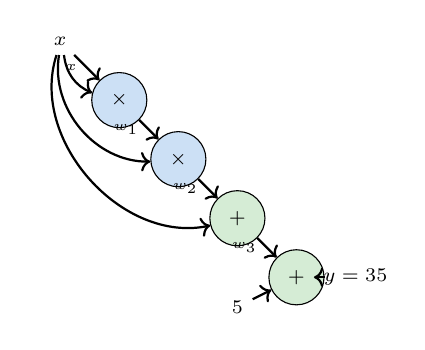
\begin{tikzpicture}[scale=0.75,
  gate/.style={draw,circle,minimum size=0.7cm,font=\scriptsize\bfseries,inner sep=0}]
  \node[font=\scriptsize] (x) at (0,4) {$x$};
  \node[gate,fill=mlblue!20] (m1) at (1,3) {$\times$};
  \node[gate,fill=mlblue!20] (m2) at (2,2) {$\times$};
  \node[gate,fill=mlgreen!20] (a1) at (3,1) {$+$};
  \node[gate,fill=mlgreen!20] (a2) at (4,0) {$+$};
  \node[font=\scriptsize] (five) at (3,-0.5) {$5$};
  \node[font=\scriptsize] (out) at (5,0) {$y=35$};
  \draw[->,thick] (x) -- (m1) node[midway,left,font=\tiny] {$x$};
  \draw[->,thick] (x) to[bend right=30] (m1);
  \draw[->,thick] (m1) -- (m2) node[midway,left,font=\tiny] {$w_1$};
  \draw[->,thick] (x) to[bend right=50] (m2);
  \draw[->,thick] (m2) -- (a1) node[midway,left,font=\tiny] {$w_2$};
  \draw[->,thick] (x) to[bend right=60] (a1);
  \draw[->,thick] (a1) -- (a2) node[midway,left,font=\tiny] {$w_3$};
  \draw[->,thick] (five) -- (a2);
  \draw[->,thick] (a2) -- (out);
\end{tikzpicture}
\end{center}
\vspace{2mm}
\footnotesize
\textbf{Circuit size} = number of multiplication gates. This circuit has 2 multiplication gates $\Rightarrow$ 2 constraints.
\end{columns}
\bottomnote{Arithmetic circuits are the universal representation -- any NP statement can be expressed as a circuit over $\mathbb{F}_p$}
\end{frame}

% Frame 11: R1CS
\begin{frame}{From Circuits to R1CS}
\begin{columns}[T]
\column{0.55\textwidth}
\begin{block}{Rank-1 Constraint System}
\footnotesize
Each multiplication gate becomes a constraint:
\[
\vec{a}_i \cdot \vec{s} \times \vec{b}_i \cdot \vec{s} = \vec{c}_i \cdot \vec{s}
\]
where $\vec{s} = (1, x, w_1, w_2, w_3, y)$ is the witness vector and $\vec{a}_i, \vec{b}_i, \vec{c}_i$ are coefficient vectors.
\end{block}
\vspace{1mm}
\begin{exampleblock}{\footnotesize Example Constraints ($x^3 + x + 5 = 35$)}
\footnotesize
\begin{align*}
\text{Gate 1:}\quad & x \times x = w_1 \\
\text{Gate 2:}\quad & w_1 \times x = w_2 \\
\text{Gate 3:}\quad & (w_2 + x) \times 1 = w_3 \\
\text{Gate 4:}\quad & (w_3 + 5) \times 1 = y
\end{align*}
\end{exampleblock}

\column{0.45\textwidth}
\begin{block}{Matrix Form}
\footnotesize
$\vec{s} = (1, x, w_1, w_2, w_3, y)$

\vspace{2mm}
$A \cdot \vec{s} \circ B \cdot \vec{s} = C \cdot \vec{s}$

\vspace{2mm}
where $A$, $B$, $C$ are sparse matrices encoding the left input, right input, and output of each gate.
\end{block}
\vspace{2mm}
\begin{alertblock}{\footnotesize Why R1CS Matters}
\footnotesize
R1CS is the intermediate representation between:
\begin{itemize}
  \item High-level programs (Circom, Noir)
  \item Low-level proof systems (Groth16, PLONK)
\end{itemize}
The compiler chain: Code $\rightarrow$ Circuit $\rightarrow$ R1CS $\rightarrow$ QAP $\rightarrow$ Proof.
\end{alertblock}
\end{columns}
\bottomnote{R1CS reduces any computation to a system of quadratic equations -- the standard input format for SNARKs}
\end{frame}

% Frame 12: QAP
\begin{frame}{QAP: Quadratic Arithmetic Programs}
\begin{columns}[T]
\column{0.55\textwidth}
\begin{block}{From R1CS to Polynomials}
\footnotesize
Transform each column of $A$, $B$, $C$ matrices into polynomials via \textbf{Lagrange interpolation}:
\[
A_j(x),\ B_j(x),\ C_j(x) \quad \text{for } j = 1, \ldots, m
\]
where $m$ is the number of witness variables.
\end{block}
\vspace{1mm}
\begin{block}{QAP Equation}
\footnotesize
Define:
\begin{align*}
A(x) &= \sum_j s_j \cdot A_j(x) \\
B(x) &= \sum_j s_j \cdot B_j(x) \\
C(x) &= \sum_j s_j \cdot C_j(x)
\end{align*}
The R1CS is satisfied iff:
\[
\boxed{A(x) \cdot B(x) - C(x) = H(x) \cdot Z(x)}
\]
where $Z(x) = \prod_{i=1}^{n} (x - \omega^i)$ is the vanishing polynomial.
\end{block}

\column{0.45\textwidth}
\begin{block}{Key Insight}
\footnotesize
Checking $n$ constraints in R1CS reduces to checking \textbf{one polynomial equation}. This is what makes SNARKs succinct!
\end{block}
\vspace{2mm}
\begin{exampleblock}{\footnotesize Why Polynomials?}
\footnotesize
\begin{itemize}
  \item Polynomials of degree $d$ are determined by $d+1$ points
  \item Two different polynomials of degree $d$ agree on at most $d$ points
  \item Checking at a random point: soundness error $\leq d/|\mathbb{F}|$ (Schwartz-Zippel)
\end{itemize}
\end{exampleblock}
\vspace{2mm}
\begin{block}{Schwartz-Zippel Lemma}
\footnotesize
If $p(x) \not\equiv 0$ and $\deg(p) = d$:
\[
\Pr_{r \leftarrow \mathbb{F}}[p(r) = 0] \leq \frac{d}{|\mathbb{F}|}
\]
\end{block}
\end{columns}
\bottomnote{QAP converts constraint checking into polynomial identity testing -- the mathematical heart of SNARKs}
\end{frame}

% Frame 13: Information-Theoretic vs Computational Security
\begin{frame}{Information-Theoretic vs Computational Security}
\begin{columns}[T]
\column{0.5\textwidth}
\begin{block}{Information-Theoretic Security}
\footnotesize
\begin{itemize}
  \item Secure against \textbf{unbounded} adversaries
  \item No computational assumptions needed
  \item Security holds even with infinite computing power
  \item Example: one-time pad, Pedersen hiding
\end{itemize}
\end{block}
\vspace{2mm}
\begin{block}{Computational Security}
\footnotesize
\begin{itemize}
  \item Secure against \textbf{PPT} (probabilistic polynomial-time) adversaries
  \item Relies on hardness assumptions (DLog, pairings)
  \item Could be broken with sufficient computation
  \item Example: RSA, ECDSA, most ZK systems
\end{itemize}
\end{block}

\column{0.5\textwidth}
\footnotesize
\begin{tabular}{lcc}
\toprule
\textbf{System} & \textbf{ZK Type} & \textbf{Soundness} \\
\midrule
Schnorr & SHVZK (comp.) & Comp. \\
Groth16 & Comp. ZK & Comp. \\
Bulletproofs & Perf. SHVZK & Comp. \\
STARKs & Comp. ZK & Info-theoretic \\
\bottomrule
\end{tabular}
\vspace{3mm}
\begin{alertblock}{\footnotesize Post-Quantum Implications}
\footnotesize
\begin{itemize}
  \item Computationally secure systems based on DLog/pairings are broken by quantum computers
  \item STARKs use hash functions only $\Rightarrow$ post-quantum secure
  \item SNARKs need pairing-friendly curves $\Rightarrow$ quantum-vulnerable
\end{itemize}
\end{alertblock}
\end{columns}
\bottomnote{The security model determines what adversaries a system can withstand -- critical for long-term protocol design}
\end{frame}

% Frame 14: Section 1 Summary
\begin{frame}{Section 1 Summary: ZK Foundations}
\begin{columns}[T]
\column{0.5\textwidth}
\begin{block}{Key Concepts}
\footnotesize
\begin{enumerate}
  \item ZK proofs: completeness, soundness, zero-knowledge
  \item Simulation paradigm proves zero-knowledge property
  \item Pedersen commitments: perfectly hiding, computationally binding
  \item Schnorr protocol: 3-move sigma protocol for DLog
  \item KZG: polynomial commitment via pairings
\end{enumerate}
\end{block}

\column{0.5\textwidth}
\begin{block}{Mathematical Toolkit}
\footnotesize
\begin{align}
C_{\text{Pedersen}} &= g^v \cdot h^r \\
\text{Schnorr verify:}\quad g^z &= a \cdot y^e \\
C_{\text{KZG}} &= [p(s)]_1 \\
\text{R1CS:}\quad \vec{a} \cdot \vec{s} \times \vec{b} \cdot \vec{s} &= \vec{c} \cdot \vec{s} \\
\text{QAP:}\quad A \cdot B - C &= H \cdot Z
\end{align}
\end{block}
\vspace{2mm}
\begin{exampleblock}{\footnotesize Next Section}
\footnotesize
$\Rightarrow$ \textbf{Proof Systems:} Groth16, PLONK, STARKs, Bulletproofs -- how they work and how they compare.
\end{exampleblock}
\end{columns}
\bottomnote{These mathematical primitives are the building blocks for all modern proof systems covered next}
\end{frame}

%% ============================================================
%% SECTION 2: PROOF SYSTEMS -- SNARKs, STARKs, BULLETPROOFS
%% ============================================================
\section{Proof Systems -- SNARKs, STARKs, Bulletproofs}

% Frame 15: Taxonomy
\begin{frame}{Taxonomy of ZK Proof Systems}
\begin{center}
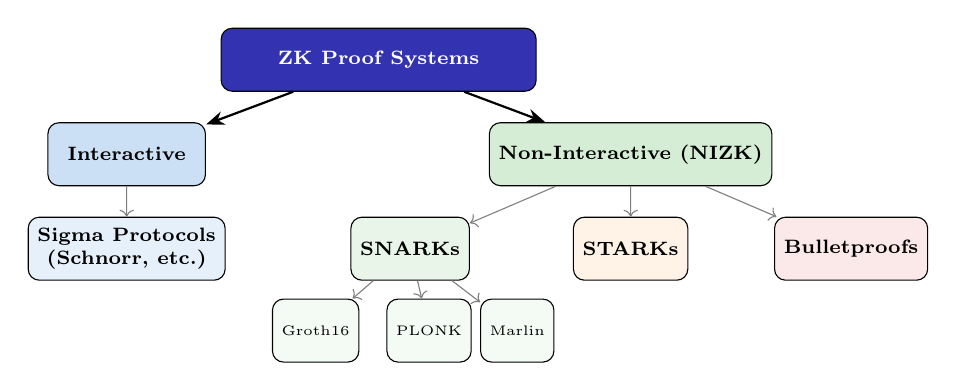
\begin{tikzpicture}[scale=0.8,
  bx/.style={draw,rounded corners=4pt,minimum height=0.8cm,align=center,font=\scriptsize\bfseries}]
  \node[bx,fill=mlpurple,text=white,minimum width=4cm] (root) at (5,4) {ZK Proof Systems};
  \node[bx,fill=mlblue!20,minimum width=2cm] (int) at (1,2.5) {Interactive};
  \node[bx,fill=mlgreen!20,minimum width=2cm] (nizk) at (9,2.5) {Non-Interactive (NIZK)};
  \node[bx,fill=mlblue!10] (sigma) at (1,1) {Sigma Protocols\\(Schnorr, etc.)};
  \node[bx,fill=mlgreen!10] (snark) at (5.5,1) {SNARKs};
  \node[bx,fill=mlorange!10] (stark) at (9,1) {STARKs};
  \node[bx,fill=mlred!10] (bp) at (12.5,1) {Bulletproofs};
  \node[bx,fill=mlgreen!5,font=\tiny] (g16) at (4,-0.3) {Groth16};
  \node[bx,fill=mlgreen!5,font=\tiny] (plonk) at (5.8,-0.3) {PLONK};
  \node[bx,fill=mlgreen!5,font=\tiny] (marlin) at (7.2,-0.3) {Marlin};
  \draw[-{Stealth},thick] (root) -- (int);
  \draw[-{Stealth},thick] (root) -- (nizk);
  \draw[->,mlgray] (int) -- (sigma);
  \draw[->,mlgray] (nizk) -- (snark);
  \draw[->,mlgray] (nizk) -- (stark);
  \draw[->,mlgray] (nizk) -- (bp);
  \draw[->,mlgray] (snark) -- (g16);
  \draw[->,mlgray] (snark) -- (plonk);
  \draw[->,mlgray] (snark) -- (marlin);
\end{tikzpicture}
\end{center}
\vspace{1mm}
\footnotesize
\begin{tabular}{lcccl}
\toprule
\textbf{Key Differentiator} & \textbf{SNARKs} & \textbf{STARKs} & \textbf{Bulletproofs} & \textbf{Trade-off} \\
\midrule
Trusted Setup & Yes & No & No & Trust vs transparency \\
Proof Size & \textasciitilde200B & \textasciitilde45KB & \textasciitilde1.5KB & Bandwidth cost \\
Verification & O(1) & O(log$^2$ n) & O(n) & On-chain cost \\
Post-Quantum & No & Yes & No & Future-proofing \\
\bottomrule
\end{tabular}
\bottomnote{No single system dominates -- each makes different trade-offs between trust, size, and quantum resistance}
\end{frame}

% Frame 16: Groth16
\begin{frame}{Groth16: The Classic SNARK}
\begin{columns}[T]
\column{0.55\textwidth}
\begin{block}{Core Idea (Groth, 2016)}
\footnotesize
Given a QAP: $A(x) \cdot B(x) - C(x) = H(x) \cdot Z(x)$

The prover produces a proof $\pi = (A, B, C) \in \mathbb{G}_1 \times \mathbb{G}_2 \times \mathbb{G}_1$ (3 group elements, \textasciitilde200 bytes).
\end{block}
\vspace{1mm}
\begin{block}{Verification Equation}
\footnotesize
\[
e(A, B) = e(\alpha, \beta) \cdot e\!\left(\sum_i x_i \cdot [L_i]_1,\ [\gamma]_2\right) \cdot e(C, \delta)
\]
where $e: \mathbb{G}_1 \times \mathbb{G}_2 \rightarrow \mathbb{G}_T$ is a bilinear pairing.
\end{block}
\vspace{1mm}
\begin{alertblock}{\footnotesize Per-Circuit Setup}
\footnotesize
Groth16 requires a \textbf{new trusted setup for each circuit}. Change the program $\Rightarrow$ new ceremony required.
\end{alertblock}

\column{0.45\textwidth}
\footnotesize
\begin{tabular}{ll}
\toprule
\textbf{Metric} & \textbf{Value} \\
\midrule
Proof size & 3 group elements (\textasciitilde192B) \\
Verification & 3 pairings (\textasciitilde1ms) \\
Prover time & O($n \log n$) \\
CRS size & O($n$) \\
Security & Comp.\ (q-type assumptions) \\
\bottomrule
\end{tabular}
\vspace{3mm}
\begin{exampleblock}{\footnotesize Used By}
\footnotesize
\begin{itemize}
  \item Zcash (Sapling circuit)
  \item Tornado Cash
  \item Filecoin
  \item Many early ZK projects
\end{itemize}
\end{exampleblock}
\end{columns}
\bottomnote{Groth16 remains the most efficient SNARK for verification -- but per-circuit setup is a major drawback}
\end{frame}

% Frame 17: Trusted Setup Ceremony
\begin{frame}{The Trusted Setup Ceremony}
\begin{columns}[T]
\column{0.55\textwidth}
\begin{block}{Multi-Party Computation (MPC)}
\footnotesize
\begin{enumerate}
  \item Each participant $i$ samples random $\tau_i$
  \item Computes $\text{SRS}_i = \text{SRS}_{i-1}^{\tau_i}$
  \item Destroys $\tau_i$ (the ``toxic waste'')
  \item Passes $\text{SRS}_i$ to next participant
\end{enumerate}
\end{block}
\vspace{2mm}
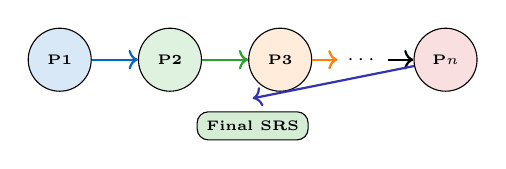
\begin{tikzpicture}[scale=0.7]
  \node[draw,fill=mlblue!15,circle,minimum size=0.8cm,font=\tiny\bfseries] (p1) at (0,0) {P1};
  \node[draw,fill=mlgreen!15,circle,minimum size=0.8cm,font=\tiny\bfseries] (p2) at (2,0) {P2};
  \node[draw,fill=mlorange!15,circle,minimum size=0.8cm,font=\tiny\bfseries] (p3) at (4,0) {P3};
  \node[font=\scriptsize] (dots) at (5.5,0) {$\cdots$};
  \node[draw,fill=mlred!15,circle,minimum size=0.8cm,font=\tiny\bfseries] (pn) at (7,0) {P$n$};
  \draw[->,thick,mlblue] (p1) -- (p2);
  \draw[->,thick,mlgreen] (p2) -- (p3);
  \draw[->,thick,mlorange] (p3) -- (dots);
  \draw[->,thick] (dots) -- (pn);
  \node[draw,fill=mlgreen!20,rounded corners,font=\tiny\bfseries,align=center] at (3.5,-1.2) {Final SRS};
  \draw[->,thick,mlpurple] (pn) -- (3.5,-0.7);
\end{tikzpicture}

\column{0.45\textwidth}
\begin{block}{Security Guarantee}
\footnotesize
\textbf{1-of-$n$ honest:} If \textit{at least one} participant honestly destroys their $\tau_i$, the setup is secure.
\end{block}
\vspace{2mm}
\begin{alertblock}{\footnotesize The Risk}
\footnotesize
If ALL participants collude (know combined $\tau$), they can:
\begin{itemize}
  \item Forge proofs for false statements
  \item Counterfeit tokens in Zcash
  \item Completely break soundness
\end{itemize}
\end{alertblock}
\vspace{2mm}
\begin{exampleblock}{\footnotesize Powers of Tau}
\footnotesize
Zcash Sprout: 6 participants (2016)\\
Zcash Sapling: 90 participants (2018)\\
Perpetual Powers of Tau: 1000+ (ongoing)
\end{exampleblock}
\end{columns}
\bottomnote{``Don't trust, verify'' -- except for the trusted setup, where you must trust at least one participant was honest}
\end{frame}

% Frame 18: PLONK
\begin{frame}{PLONK: Universal SNARKs}
\begin{columns}[T]
\column{0.55\textwidth}
\begin{block}{Key Innovation}
\footnotesize
\textbf{Universal SRS:} One trusted setup works for \textit{all circuits} up to a maximum size. No per-circuit ceremony!
\end{block}
\vspace{1mm}
\begin{block}{Gate Equation}
\footnotesize
PLONK uses a single arithmetic gate:
\[
q_L \cdot a + q_R \cdot b + q_O \cdot c + q_M \cdot a \cdot b + q_C = 0
\]
where $q_L, q_R, q_O, q_M, q_C$ are selector polynomials.
\begin{itemize}
  \item Addition: $q_L = q_R = 1, q_O = -1, q_M = 0$
  \item Multiplication: $q_M = 1, q_O = -1, q_L = q_R = 0$
\end{itemize}
\end{block}

\column{0.45\textwidth}
\begin{block}{Copy Constraints}
\footnotesize
Wiring between gates is enforced via \textbf{permutation polynomials}:
\[
\sigma: \{1, \ldots, 3n\} \rightarrow \{1, \ldots, 3n\}
\]
Grand product argument checks:
\[
\prod_{i} \frac{f(i)}{g(\sigma(i))} = 1
\]
\end{block}
\vspace{2mm}
\begin{exampleblock}{\footnotesize Advantages over Groth16}
\footnotesize
\begin{itemize}
  \item Universal setup (reusable)
  \item Updatable (new participants can strengthen)
  \item Custom gates for efficiency
  \item Used by: Aztec, Scroll, Polygon zkEVM
\end{itemize}
\end{exampleblock}
\end{columns}
\bottomnote{PLONK (2019) made universal SNARKs practical -- one ceremony rules them all}
\end{frame}

% Frame 19: STARKs
\begin{frame}{STARKs: Transparent Proofs}
\begin{columns}[T]
\column{0.55\textwidth}
\begin{block}{Key Properties}
\footnotesize
\begin{itemize}
  \item \textbf{No trusted setup} -- uses only hash functions (public randomness)
  \item \textbf{Post-quantum secure} -- no elliptic curves or pairings
  \item \textbf{Scalable prover:} quasi-linear $O(n \log n)$
  \item Proof size: $O(\log^2 n)$ -- larger than SNARKs
\end{itemize}
\end{block}
\vspace{1mm}
\begin{block}{Architecture}
\footnotesize
\begin{enumerate}
  \item \textbf{Arithmetization:} Encode computation as polynomial constraints (AIR -- Algebraic Intermediate Representation)
  \item \textbf{Low Degree Testing:} Prove polynomial has low degree via FRI
  \item \textbf{Commitment:} Merkle tree over evaluations (hash-based)
\end{enumerate}
\end{block}

\column{0.45\textwidth}
\footnotesize
\begin{tabular}{ll}
\toprule
\textbf{Metric} & \textbf{Value} \\
\midrule
Proof size & 45--200 KB \\
Verification & O($\log^2 n$) \\
Prover time & O($n \log n$) \\
Setup & None (transparent) \\
Quantum safe & Yes \\
\bottomrule
\end{tabular}
\vspace{3mm}
\begin{exampleblock}{\footnotesize Used By}
\footnotesize
\begin{itemize}
  \item StarkNet (Ethereum L2)
  \item StarkEx (dYdX, Sorare)
  \item Cairo programming language
  \item Polygon Miden
\end{itemize}
\end{exampleblock}
\vspace{2mm}
\begin{block}{Trade-off}
\footnotesize
Larger proofs $\Rightarrow$ higher on-chain cost. Mitigated by STARK-to-SNARK wrapping (``proof compression'').
\end{block}
\end{columns}
\bottomnote{STARKs trade proof size for transparency and quantum resistance -- invented by Eli Ben-Sasson (StarkWare)}
\end{frame}

% Frame 20: FRI Protocol
\begin{frame}{FRI Protocol Deep Dive}
\begin{columns}[T]
\column{0.55\textwidth}
\begin{block}{Fast Reed-Solomon IOP (FRI)}
\footnotesize
Goal: Prove that a function $f: D \rightarrow \mathbb{F}$ is ``close to'' a polynomial of degree $< d$.
\end{block}
\vspace{1mm}
\begin{block}{Folding Procedure}
\footnotesize
Split polynomial into even and odd parts:
\[
p(x) = p_{\text{even}}(x^2) + x \cdot p_{\text{odd}}(x^2)
\]
Given random $\alpha$ from verifier:
\[
p'(y) = p_{\text{even}}(y) + \alpha \cdot p_{\text{odd}}(y)
\]
New polynomial $p'$ has \textbf{half the degree}!
\end{block}
\vspace{1mm}
\begin{exampleblock}{\footnotesize Recursive Folding}
\footnotesize
Repeat $\log_2 d$ times: $d \rightarrow d/2 \rightarrow d/4 \rightarrow \cdots \rightarrow 1$

Final check: is $p'$ a constant polynomial?
\end{exampleblock}

\column{0.45\textwidth}
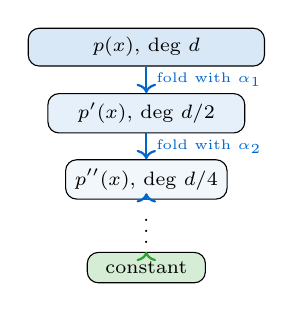
\begin{tikzpicture}[scale=0.7]
  \node[draw,fill=mlblue!15,rounded corners,minimum width=3cm,font=\scriptsize,align=center] (d0) at (0,4) {$p(x)$, deg $d$};
  \node[draw,fill=mlblue!10,rounded corners,minimum width=2.5cm,font=\scriptsize,align=center] (d1) at (0,2.8) {$p'(x)$, deg $d/2$};
  \node[draw,fill=mlblue!5,rounded corners,minimum width=2cm,font=\scriptsize,align=center] (d2) at (0,1.6) {$p''(x)$, deg $d/4$};
  \node[font=\scriptsize] (dots) at (0,0.8) {$\vdots$};
  \node[draw,fill=mlgreen!20,rounded corners,minimum width=1.5cm,font=\scriptsize,align=center] (df) at (0,0) {constant};
  \draw[->,thick,mlblue] (d0) -- (d1) node[midway,right,font=\tiny] {fold with $\alpha_1$};
  \draw[->,thick,mlblue] (d1) -- (d2) node[midway,right,font=\tiny] {fold with $\alpha_2$};
  \draw[->,thick,mlblue] (d2) -- (dots);
  \draw[->,thick,mlgreen] (dots) -- (df);
\end{tikzpicture}
\vspace{2mm}
\begin{block}{Verification}
\footnotesize
\begin{itemize}
  \item Merkle path checks on evaluations
  \item Consistency checks between layers
  \item Total: $O(\log^2 d)$ field operations
\end{itemize}
\end{block}
\end{columns}
\bottomnote{FRI is the polynomial commitment scheme for STARKs -- it replaces pairings with hash-based Merkle proofs}
\end{frame}

% Frame 21: Bulletproofs
\begin{frame}{Bulletproofs: No Trusted Setup, Small Proofs}
\begin{columns}[T]
\column{0.55\textwidth}
\begin{block}{Inner Product Argument}
\footnotesize
Prove knowledge of vectors $\vec{a}, \vec{b} \in \mathbb{F}^n$ such that:
\[
\langle \vec{a}, \vec{b} \rangle = c \quad \text{and} \quad P = \vec{g}^{\vec{a}} \cdot \vec{h}^{\vec{b}} \cdot u^c
\]
\end{block}
\vspace{1mm}
\begin{block}{Recursive Halving}
\footnotesize
Split vectors: $\vec{a} = (\vec{a}_L, \vec{a}_R)$, $\vec{b} = (\vec{b}_L, \vec{b}_R)$

Compute cross-terms $L, R$ and fold with challenge $x$:
\begin{align*}
\vec{a}' &= x \cdot \vec{a}_L + x^{-1} \cdot \vec{a}_R \\
\vec{b}' &= x^{-1} \cdot \vec{b}_L + x \cdot \vec{b}_R
\end{align*}
After $\log_2 n$ rounds: vectors reduce to scalars.
\end{block}

\column{0.45\textwidth}
\begin{block}{Proof Size}
\footnotesize
$2 \log_2 n$ group elements $\approx O(\log n)$

For $n = 64$ (range proof): $\approx 672$ bytes.
\end{block}
\vspace{2mm}
\begin{block}{Range Proofs}
\footnotesize
Prove $v \in [0, 2^n)$ without revealing $v$:
\begin{itemize}
  \item Express $v$ in binary: $v = \sum_{i} b_i \cdot 2^i$
  \item Prove each $b_i \in \{0, 1\}$
  \item Inner product argument on binary decomposition
\end{itemize}
\end{block}
\vspace{2mm}
\begin{exampleblock}{\footnotesize Used By}
\footnotesize
\begin{itemize}
  \item Monero (confidential amounts)
  \item Mimblewimble (Grin, Beam)
\end{itemize}
\end{exampleblock}
\end{columns}
\bottomnote{Bulletproofs: no trusted setup, logarithmic proof size, but linear verification -- ideal for range proofs in privacy coins}
\end{frame}

% Frame 22: Comparison Table
\begin{frame}{Proof Systems Comparison}
\footnotesize
\begin{tabular}{lccccc}
\toprule
\textbf{Property} & \textbf{Groth16} & \textbf{PLONK} & \textbf{STARKs} & \textbf{Bulletproofs} \\
\midrule
Trusted Setup & Per-circuit & Universal & None & None \\
Proof Size & \textasciitilde200B & \textasciitilde400B & 45--200KB & $O(\log n)$ \\
Verification & O(1), 3 pairings & O(1), 1 pairing & O($\log^2 n$) & O($n$) \\
Prover Time & O($n \log n$) & O($n \log n$) & O($n \log n$) & O($n^2$) \\
Quantum Safe & No & No & Yes & No \\
Assumptions & q-type & AGM + ROM & CRHF only & DLog \\
\midrule
Used By & Zcash, Filecoin & Aztec, Scroll & StarkNet, dYdX & Monero, Grin \\
\bottomrule
\end{tabular}
\vspace{3mm}
\begin{columns}[T]
\column{0.5\textwidth}
\begin{exampleblock}{\footnotesize Choosing a System}
\footnotesize
\begin{itemize}
  \item Minimise on-chain cost $\rightarrow$ Groth16 or PLONK
  \item No trust assumptions $\rightarrow$ STARKs
  \item Range proofs only $\rightarrow$ Bulletproofs
  \item Future-proof $\rightarrow$ STARKs
\end{itemize}
\end{exampleblock}

\column{0.5\textwidth}
\begin{block}{\footnotesize Hybrid Approaches}
\footnotesize
\begin{itemize}
  \item \textbf{STARK-to-SNARK:} Prove STARK, wrap in SNARK for small on-chain proof (Polygon zkEVM)
  \item \textbf{Recursive SNARKs:} Prove verification of previous proof (Nova, Halo)
\end{itemize}
\end{block}
\end{columns}
\bottomnote{The ``proof system wars'' are driving rapid innovation -- hybrid approaches combine the best of each}
\end{frame}

% Frame 23: Recursive Proofs
\begin{frame}{Recursive Proofs \& Proof Composition}
\begin{columns}[T]
\column{0.55\textwidth}
\begin{block}{Concept}
\footnotesize
A \textbf{recursive proof} proves that another proof is valid inside itself. The verifier of proof $n$ becomes part of the circuit for proof $n+1$.
\end{block}
\vspace{1mm}
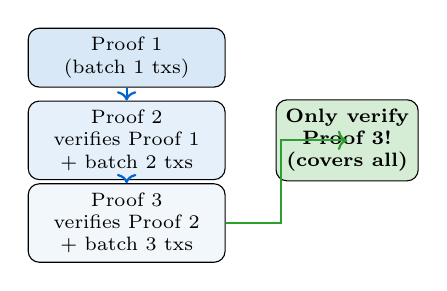
\begin{tikzpicture}[scale=0.7]
  \node[draw,fill=mlblue!15,rounded corners,minimum width=2.5cm,font=\scriptsize,align=center] (p1) at (0,3) {Proof 1\\(batch 1 txs)};
  \node[draw,fill=mlblue!10,rounded corners,minimum width=2.5cm,font=\scriptsize,align=center] (p2) at (0,1.5) {Proof 2\\verifies Proof 1\\+ batch 2 txs};
  \node[draw,fill=mlblue!5,rounded corners,minimum width=2.5cm,font=\scriptsize,align=center] (p3) at (0,0) {Proof 3\\verifies Proof 2\\+ batch 3 txs};
  \draw[->,thick,mlblue] (p1) -- (p2);
  \draw[->,thick,mlblue] (p2) -- (p3);
  \node[draw,fill=mlgreen!20,rounded corners,font=\scriptsize\bfseries,align=center] at (4,1.5) {Only verify\\Proof 3!\\(covers all)};
  \draw[->,thick,mlgreen] (p3.east) -- ++(1,0) |- (4,1.5);
\end{tikzpicture}

\column{0.45\textwidth}
\begin{block}{IVC (Incrementally Verifiable Computation)}
\footnotesize
\[
\pi_n = \text{Prove}(\text{Verify}(\pi_{n-1}) \wedge F(s_{n-1}) = s_n)
\]
Each step proves both the computation AND the validity of the previous proof.
\end{block}
\vspace{2mm}
\begin{block}{Nova Folding Scheme}
\footnotesize
Instead of full recursion, \textbf{fold} instances together:
\begin{itemize}
  \item No expensive verification inside the circuit
  \item Linear-time folding operation
  \item Final proof at the end only
  \item Dramatically reduces prover cost
\end{itemize}
\end{block}
\vspace{2mm}
\begin{exampleblock}{\footnotesize Applications}
\footnotesize
Blockchain light clients, rollup proof aggregation, long-running computations.
\end{exampleblock}
\end{columns}
\bottomnote{Recursive proofs enable unbounded computation verification with constant-size proofs -- the holy grail of ZK}
\end{frame}

% Frame 24: Groth16 Verifier in Solidity
\begin{frame}[fragile]{ZK Proof Verification in Solidity}
\begin{lstlisting}
// SPDX-License-Identifier: MIT
pragma solidity ^0.8.20;

contract Groth16Verifier {
    // Verification key (set during deployment)
    uint256[2] public alfa1;    // G1 point
    uint256[2][2] public beta2; // G2 point
    uint256[2][2] public gamma2;
    uint256[2][2] public delta2;

    struct Proof {
        uint256[2] a;    // G1
        uint256[2][2] b; // G2
        uint256[2] c;    // G1
    }

    // Verify a Groth16 proof via ecPairing precompile
    function verifyProof(
        Proof memory proof,
        uint256[] memory pubInputs
    ) public view returns (bool) {
        // Compute linear combination of public inputs
        uint256[2] memory vk_x = computeLinearCombination(pubInputs);
        // Pairing check: e(A, B) == e(alpha, beta) * e(vk_x, gamma) * e(C, delta)
        // Uses EVM precompile at address 0x08
        return pairingCheck(proof, vk_x);
    }

    function pairingCheck(Proof memory p, uint256[2] memory vk_x)
        internal view returns (bool) {
        // Encode 4 pairing pairs and call ecPairing precompile
        // Returns true if product of pairings equals 1 in G_T
        assembly { /* pairing precompile call at 0x08 */ }
        return true; // simplified
    }
}
\end{lstlisting}
\bottomnote{EVM precompiles (0x06-0x08) enable efficient elliptic curve operations needed for on-chain ZK verification}
\end{frame}

% Frame 25: Section 2 Summary
\begin{frame}{Section 2 Summary: Proof Systems}
\begin{columns}[T]
\column{0.5\textwidth}
\begin{block}{Key Concepts}
\footnotesize
\begin{enumerate}
  \item Groth16: smallest proofs, per-circuit setup
  \item PLONK: universal setup, custom gates
  \item STARKs: transparent, post-quantum, hash-based
  \item Bulletproofs: no setup, log-size, range proofs
  \item FRI: degree testing via polynomial folding
  \item Recursive proofs: verify proofs inside proofs
\end{enumerate}
\end{block}

\column{0.5\textwidth}
\begin{block}{Design Decision Guide}
\footnotesize
\begin{itemize}
  \item[\textcolor{mlblue}{$\bullet$}] On-chain verification cost critical? $\rightarrow$ SNARK
  \item[\textcolor{mlgreen}{$\bullet$}] No trust assumptions? $\rightarrow$ STARK
  \item[\textcolor{mlorange}{$\bullet$}] Quantum resistance needed? $\rightarrow$ STARK
  \item[\textcolor{mlred}{$\bullet$}] Privacy coin amounts? $\rightarrow$ Bulletproofs
  \item[\textcolor{mlpurple}{$\bullet$}] Flexibility + reusable setup? $\rightarrow$ PLONK
\end{itemize}
\end{block}
\vspace{2mm}
\begin{exampleblock}{\footnotesize Next Section}
\footnotesize
$\Rightarrow$ \textbf{Privacy Coins:} How Monero and Zcash use these proof systems for transaction privacy.
\end{exampleblock}
\end{columns}
\bottomnote{The proof system landscape is evolving rapidly -- new systems like Lasso and HyperNova push boundaries further}
\end{frame}

%% ===== SECTION 3: Privacy Coins -- Monero, Zcash, Comparison =====
\section{Privacy Coins}

% Frame 26: Pseudonymity vs Anonymity
\begin{frame}{The Privacy Spectrum in Blockchain}
\begin{columns}[T]
\column{0.55\textwidth}
\begin{block}{\footnotesize Pseudonymity (Bitcoin, Ethereum)}
\footnotesize
\begin{itemize}
\item Addresses are \textbf{pseudonyms}, not identities
\item All transactions publicly visible on-chain
\item Chain analysis can \textbf{link} addresses to identities
\item Heuristics: common input ownership, change detection
\item Once one address deanonymized $\Rightarrow$ transaction graph exposed
\end{itemize}
\end{block}
\begin{alertblock}{\footnotesize Anonymity (Privacy Coins)}
\footnotesize
\begin{itemize}
\item \textbf{Sender} privacy: who sent the transaction?
\item \textbf{Receiver} privacy: who received it?
\item \textbf{Amount} privacy: how much was transferred?
\item \textbf{Unlinkability}: can transactions be connected?
\end{itemize}
\end{alertblock}
\column{0.43\textwidth}
\begin{center}
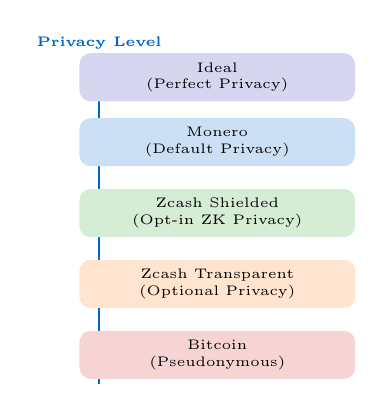
\begin{tikzpicture}[scale=0.75, every node/.style={font=\tiny}]
% Privacy spectrum
\draw[thick, ->, mlblue] (0,0) -- (0,5.5) node[above]{\textbf{Privacy Level}};
% Levels
\node[fill=mlred!20, rounded corners, minimum width=3.5cm, align=center] at (2,0.5) {Bitcoin\\(Pseudonymous)};
\node[fill=mlorange!20, rounded corners, minimum width=3.5cm, align=center] at (2,1.7) {Zcash Transparent\\(Optional Privacy)};
\node[fill=mlgreen!20, rounded corners, minimum width=3.5cm, align=center] at (2,2.9) {Zcash Shielded\\(Opt-in ZK Privacy)};
\node[fill=mlblue!20, rounded corners, minimum width=3.5cm, align=center] at (2,4.1) {Monero\\(Default Privacy)};
\node[fill=mlpurple!20, rounded corners, minimum width=3.5cm, align=center] at (2,5.2) {Ideal\\(Perfect Privacy)};
\end{tikzpicture}
\end{center}
\end{columns}
\bottomnote{Chain analysis firms (Chainalysis, Elliptic) can deanonymize most Bitcoin transactions}
\end{frame}

% Frame 27: Ring Signatures
\begin{frame}{Ring Signatures: Hiding the Sender}
\begin{columns}[T]
\column{0.52\textwidth}
\begin{block}{\footnotesize Definition (Rivest, Shamir, Tauman 2001)}
\footnotesize
A \textbf{ring signature} allows a signer to produce a signature on behalf of an ad-hoc group (``ring'') without revealing \emph{which} member signed.
\end{block}
\vspace{0.1cm}
\footnotesize
\textbf{Construction:}
Given ring $R = \{pk_1, \ldots, pk_n\}$ and signer's secret key $sk_i$:
\begin{enumerate}
\item Choose random values $s_j$ for all $j \neq i$
\item Compute partial signatures: $e_j = H(m \| s_j)$ for $j \neq i$
\item Solve for $s_i$ such that the ring ``closes'':
$$\prod_{j=1}^{n} g^{s_j} \cdot pk_j^{e_j} = 1 \pmod{p}$$
\item Output $\sigma = (e_1, s_1, \ldots, s_n)$
\end{enumerate}
\column{0.46\textwidth}
\begin{center}
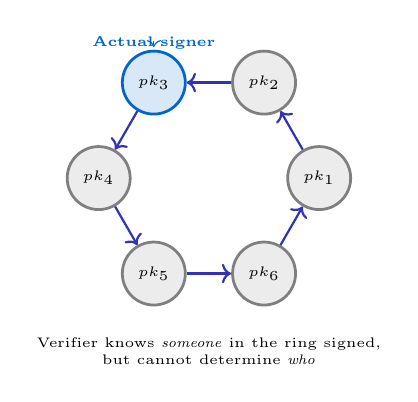
\begin{tikzpicture}[scale=0.7, every node/.style={font=\tiny}]
% Ring structure
\foreach \i/\c/\lbl in {0/mlgray/pk_1, 60/mlgray/pk_2, 120/mlblue/pk_3, 180/mlgray/pk_4, 240/mlgray/pk_5, 300/mlgray/pk_6} {
  \node[circle, draw=\c, fill=\c!15, minimum size=0.8cm, line width=1pt] (n\i) at (\i:2cm) {$\lbl$};
}
% Ring arrows
\foreach \a/\b in {0/60, 60/120, 120/180, 180/240, 240/300, 300/0} {
  \draw[->, thick, mlpurple] (n\a) -- (n\b);
}
% Label actual signer
\node[above=0.3cm, mlblue, font=\tiny\bfseries] at (n120) {Actual signer};
\draw[->, mlblue, dashed] (n120.north) ++(0,0.15) -- ++(0,-0.1);
% Caption
\node[below=0.3cm, font=\tiny, align=center] at (0,-2.3) {Verifier knows \emph{someone} in the ring signed,\\but cannot determine \emph{who}};
\end{tikzpicture}
\end{center}
\vspace{0.1cm}
\begin{exampleblock}{\footnotesize Key Properties}
\footnotesize
\begin{itemize}
\item \textbf{Unforgeability}: Only ring members can sign
\item \textbf{Anonymity}: Signer indistinguishable among ring
\item \textbf{No setup}: No group manager needed
\end{itemize}
\end{exampleblock}
\end{columns}
\bottomnote{Ring signatures provide plausible deniability -- any ring member could have been the signer}
\end{frame}

% Frame 28: Stealth Addresses
\begin{frame}{Stealth Addresses: Hiding the Receiver}
\begin{columns}[T]
\column{0.50\textwidth}
\begin{block}{\footnotesize Dual-Key Stealth Address Protocol (DKSAP)}
\footnotesize
Receiver publishes two public keys: $(A, B)$ where $A = aG$, $B = bG$.
\end{block}
\vspace{0.1cm}
\footnotesize
\textbf{Sending:}
\begin{enumerate}
\item Sender generates random $r \xleftarrow{\$} \mathbb{Z}_q$
\item Computes shared secret: $S = r \cdot A = r \cdot a \cdot G$
\item Derives one-time key: $P = H_s(S) \cdot G + B$
\item Publishes ephemeral key $R = r \cdot G$ on-chain
\item Sends funds to address derived from $P$
\end{enumerate}
\vspace{0.1cm}
\textbf{Receiving:}
\begin{enumerate}
\item Receiver scans $R$ values, computes $S' = a \cdot R$
\item Checks if $P' = H_s(S') \cdot G + B$ matches output
\item Spends with $x = H_s(S') + b$
\end{enumerate}
\column{0.48\textwidth}
\begin{center}
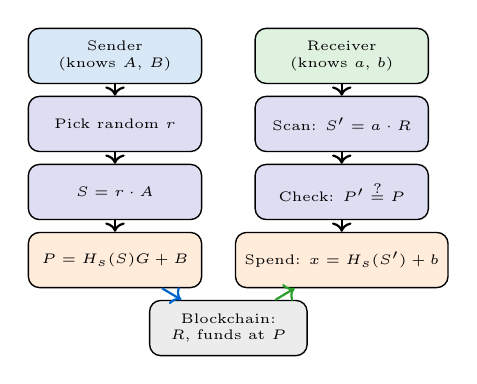
\begin{tikzpicture}[scale=0.72, every node/.style={font=\tiny},
  bx/.style={rounded corners, minimum width=2.2cm, minimum height=0.7cm, align=center, draw, line width=0.5pt}]
% Sender
\node[bx, fill=mlblue!15] (sender) at (0,4.5) {Sender\\(knows $A$, $B$)};
% Steps
\node[bx, fill=mllavender!40] (rand) at (0,3.3) {Pick random $r$};
\node[bx, fill=mllavender!40] (shared) at (0,2.1) {$S = r \cdot A$};
\node[bx, fill=mlorange!15] (otk) at (0,0.9) {$P = H_s(S)G + B$};
% Receiver
\node[bx, fill=mlgreen!15] (recv) at (4,4.5) {Receiver\\(knows $a$, $b$)};
\node[bx, fill=mllavender!40] (scan) at (4,3.3) {Scan: $S' = a \cdot R$};
\node[bx, fill=mllavender!40] (check) at (4,2.1) {Check: $P' \stackrel{?}{=} P$};
\node[bx, fill=mlorange!15] (spend) at (4,0.9) {Spend: $x = H_s(S') + b$};
% Blockchain
\node[bx, fill=mlgray!15, minimum width=2cm] (chain) at (2,-0.3) {Blockchain:\\$R$, funds at $P$};
% Arrows
\draw[->, thick] (sender) -- (rand);
\draw[->, thick] (rand) -- (shared);
\draw[->, thick] (shared) -- (otk);
\draw[->, thick, mlblue] (otk) -- (chain);
\draw[->, thick, mlgreen] (chain) -- (spend);
\draw[->, thick] (recv) -- (scan);
\draw[->, thick] (scan) -- (check);
\draw[->, thick] (check) -- (spend);
\end{tikzpicture}
\end{center}
\end{columns}
\bottomnote{Each transaction creates a unique one-time address -- no two transactions share the same destination}
\end{frame}

% Frame 29: RingCT (Ring Confidential Transactions)
\begin{frame}{RingCT: Hiding the Amount}
\begin{columns}[T]
\column{0.52\textwidth}
\begin{block}{\footnotesize Pedersen Commitments for Amounts}
\footnotesize
Commit to amount $v$ with blinding factor $r$:
$$C = r \cdot G + v \cdot H$$
where $G, H$ are independent generators (nobody knows $\log_G H$).
\end{block}
\vspace{0.1cm}
\footnotesize
\textbf{Homomorphic property ensures balance:}
$$\sum C_{\text{in}} - \sum C_{\text{out}} = r_{\Delta} \cdot G + 0 \cdot H$$
If amounts balance, the difference commits to zero.

\vspace{0.2cm}
\begin{alertblock}{\footnotesize Range Proofs (Critical)}
\footnotesize
Must prove $v \in [0, 2^{64})$ to prevent:
\begin{itemize}
\item Negative amounts (creating money from nothing)
\item Overflow attacks
\end{itemize}
Monero uses \textbf{Bulletproofs} for range proofs:\\
$\mathcal{O}(\log n)$ proof size vs $\mathcal{O}(n)$ for na\"ive approach.
\end{alertblock}
\column{0.46\textwidth}
\begin{center}
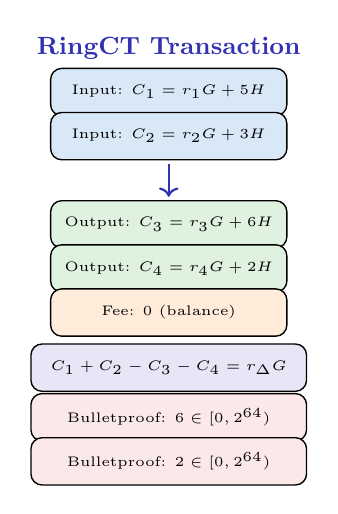
\begin{tikzpicture}[scale=0.7, every node/.style={font=\tiny},
  bx/.style={rounded corners, draw, minimum width=3cm, minimum height=0.6cm, align=center, line width=0.5pt}]
% Transaction
\node[font=\small\bfseries, mlpurple] at (2,5.5) {RingCT Transaction};
% Inputs
\node[bx, fill=mlblue!15] at (2,4.7) {Input: $C_1 = r_1G + 5H$};
\node[bx, fill=mlblue!15] at (2,3.9) {Input: $C_2 = r_2G + 3H$};
% Arrow
\draw[->, thick, mlpurple] (2,3.4) -- (2,2.8);
% Outputs
\node[bx, fill=mlgreen!15] at (2,2.3) {Output: $C_3 = r_3G + 6H$};
\node[bx, fill=mlgreen!15] at (2,1.5) {Output: $C_4 = r_4G + 2H$};
% Fee
\node[bx, fill=mlorange!15] at (2,0.7) {Fee: $0$ (balance)};
% Verification
\node[bx, fill=mllavender!30, minimum width=3.5cm] at (2,-0.3) {$C_1 + C_2 - C_3 - C_4 = r_\Delta G$};
% Range proofs
\node[bx, fill=mlred!10, minimum width=3.5cm] at (2,-1.2) {Bulletproof: $6 \in [0, 2^{64})$};
\node[bx, fill=mlred!10, minimum width=3.5cm] at (2,-2.0) {Bulletproof: $2 \in [0, 2^{64})$};
\end{tikzpicture}
\end{center}
\end{columns}
\bottomnote{RingCT was activated on Monero in January 2017 (mandatory since September 2017)}
\end{frame}

% Frame 30: Monero Architecture
\begin{frame}{Monero: Privacy by Default}
\begin{center}
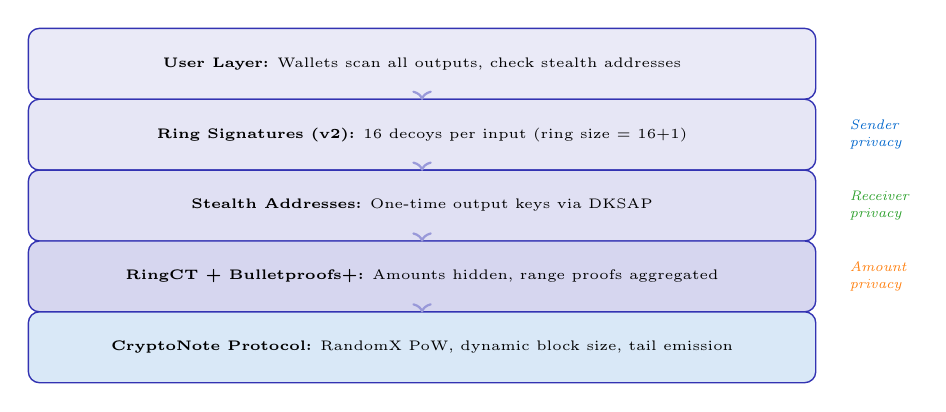
\begin{tikzpicture}[scale=0.75, every node/.style={font=\tiny},
  layer/.style={rounded corners, draw=mlpurple, minimum width=10cm, minimum height=0.9cm, align=center, line width=0.5pt}]
% Stack
\node[layer, fill=mllavender4!50] (l5) at (0,4.5) {\textbf{User Layer:} Wallets scan all outputs, check stealth addresses};
\node[layer, fill=mllavender3!50] (l4) at (0,3.3) {\textbf{Ring Signatures (v2):} 16 decoys per input (ring size = 16+1)};
\node[layer, fill=mllavender2!50] (l3) at (0,2.1) {\textbf{Stealth Addresses:} One-time output keys via DKSAP};
\node[layer, fill=mllavender!50] (l2) at (0,0.9) {\textbf{RingCT + Bulletproofs+:} Amounts hidden, range proofs aggregated};
\node[layer, fill=mlblue!15] (l1) at (0,-0.3) {\textbf{CryptoNote Protocol:} RandomX PoW, dynamic block size, tail emission};
% Arrows
\foreach \a/\b in {l1/l2, l2/l3, l3/l4, l4/l5} {
  \draw[->, thick, mlpurple!50] (\a) -- (\b);
}
% Side annotations
\node[right=0.3cm, mlblue, font=\tiny\itshape, align=left] at (l4.east) {Sender\\privacy};
\node[right=0.3cm, mlgreen, font=\tiny\itshape, align=left] at (l3.east) {Receiver\\privacy};
\node[right=0.3cm, mlorange, font=\tiny\itshape, align=left] at (l2.east) {Amount\\privacy};
\end{tikzpicture}
\end{center}
\vspace{0.1cm}
\begin{columns}[T]
\column{0.48\textwidth}
\begin{block}{\footnotesize Key Design Choices}
\footnotesize
\begin{itemize}
\item \textbf{Mandatory} privacy (no transparent pool)
\item Tail emission: 0.6 XMR/block forever
\item ASIC-resistant mining (RandomX)
\item Regular hard forks for upgrades
\end{itemize}
\end{block}
\column{0.48\textwidth}
\begin{alertblock}{\footnotesize Tradeoffs}
\footnotesize
\begin{itemize}
\item Larger transactions ($\sim$2 KB vs 250 B for BTC)
\item Wallet sync requires scanning all outputs
\item No supply auditability (hidden amounts)
\item Regulatory pressure (delisted from exchanges)
\end{itemize}
\end{alertblock}
\end{columns}
\bottomnote{Monero's ring size increased from 4 (2014) to 11 (2018) to 16 (2022) -- larger rings = stronger anonymity sets}
\end{frame}

% Frame 31: Zcash Shielded Pools
\begin{frame}{Zcash: Shielded Transaction Pools}
\begin{columns}[T]
\column{0.52\textwidth}
\begin{block}{\footnotesize Zcash Shielded Transaction Model}
\footnotesize
Zcash uses \textbf{zk-SNARKs} to prove transaction validity without revealing sender, receiver, or amount.
\end{block}
\vspace{0.1cm}
\footnotesize
\textbf{Note model} (UTXO-like):
\begin{itemize}
\item A \textbf{note} $(pk, v, \rho, rcm)$: owner, value, unique ID, randomness
\item \textbf{Note commitment}: $cm = \text{COMM}(pk \| v \| \rho; rcm)$
\item Posted to commitment tree (Merkle tree of all commitments)
\item To spend: reveal \textbf{nullifier} $nf = \text{PRF}(sk, \rho)$
\item ZK proof demonstrates:
  \begin{enumerate}
  \item Note exists in commitment tree (Merkle path valid)
  \item Spender knows secret key for the note
  \item Nullifier correctly derived (prevents double-spend)
  \item Value balance: $\sum v_{\text{in}} = \sum v_{\text{out}} + v_{\text{fee}}$
  \end{enumerate}
\end{itemize}
\column{0.46\textwidth}
\begin{center}
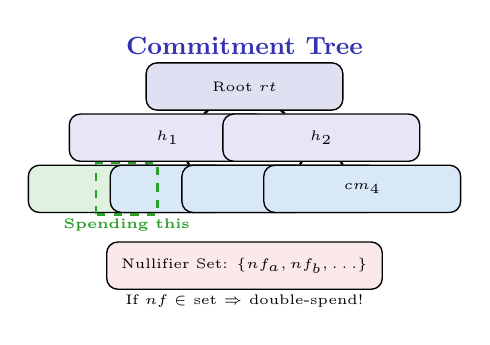
\begin{tikzpicture}[scale=0.65, every node/.style={font=\tiny},
  bx/.style={rounded corners, draw, minimum width=2.5cm, minimum height=0.6cm, align=center, line width=0.5pt}]
% Commitment tree
\node[font=\small\bfseries, mlpurple] at (2,5.5) {Commitment Tree};
% Tree root
\node[bx, fill=mlpurple!15] (root) at (2,4.7) {Root $rt$};
\node[bx, fill=mllavender!30] (h1) at (0.5,3.7) {$h_1$};
\node[bx, fill=mllavender!30] (h2) at (3.5,3.7) {$h_2$};
\node[bx, fill=mlgreen!15] (cm1) at (-0.3,2.7) {$cm_1$};
\node[bx, fill=mlblue!15] (cm2) at (1.3,2.7) {$cm_2$};
\node[bx, fill=mlblue!15] (cm3) at (2.7,2.7) {$cm_3$};
\node[bx, fill=mlblue!15] (cm4) at (4.3,2.7) {$cm_4$};
\draw[thick] (root) -- (h1);
\draw[thick] (root) -- (h2);
\draw[thick] (h1) -- (cm1);
\draw[thick] (h1) -- (cm2);
\draw[thick] (h2) -- (cm3);
\draw[thick] (h2) -- (cm4);
% Highlight spending
\draw[mlgreen, thick, dashed] (-0.9,2.2) rectangle (0.3,3.2);
\node[mlgreen, font=\tiny\bfseries] at (-0.3,2.0) {Spending this};
% Nullifier set
\node[bx, fill=mlred!10, minimum width=3.5cm] at (2,1.2) {Nullifier Set: $\{nf_a, nf_b, \ldots\}$};
\node[font=\tiny, align=center] at (2,0.5) {If $nf \in$ set $\Rightarrow$ double-spend!};
\end{tikzpicture}
\end{center}
\end{columns}
\bottomnote{Zcash processes $\sim$500K shielded transactions/month as of 2024 (Sapling + Orchard pools)}
\end{frame}

% Frame 32: Zcash Protocol Evolution
\begin{frame}{Zcash Protocol Evolution: Sprout $\to$ Sapling $\to$ Orchard}
\footnotesize
\begin{center}
\begin{adjustbox}{max width=\textwidth}
\begin{tabular}{l c c c}
\toprule
\textbf{Feature} & \textbf{Sprout (2016)} & \textbf{Sapling (2018)} & \textbf{Orchard (2022)} \\
\midrule
Proof System & Groth16 (PGHR) & \textbf{Groth16} & \textbf{Halo 2} \\
Trusted Setup & Yes (ceremony) & Yes (Powers of Tau) & \textcolor{mlgreen}{\textbf{No}} \\
Proving Time & $\sim$40 seconds & $\sim$2.3 seconds & $\sim$2.5 seconds \\
Memory Required & $\sim$3 GB & $\sim$40 MB & $\sim$40 MB \\
Curve & BN-254 & BLS12-381 & Pallas/Vesta \\
Commitment Scheme & SHA-256 compress & Pedersen hash & Sinsemilla \\
Nullifier Derivation & SHA-256 based & PRF based & Poseidon \\
Note Encryption & ECIES & In-band & In-band \\
Action Model & JoinSplit (2-in, 2-out) & Spend + Output & \textbf{Action} (unified) \\
Unified Addresses & No & No & \textcolor{mlgreen}{\textbf{Yes}} \\
\bottomrule
\end{tabular}
\end{adjustbox}
\end{center}
\vspace{0.2cm}
\begin{columns}[T]
\column{0.48\textwidth}
\begin{exampleblock}{\footnotesize Key Improvement: Halo 2}
\footnotesize
Orchard eliminates trusted setup via \textbf{recursive proof composition} on a cycle of curves (Pallas/Vesta). No toxic waste.
\end{exampleblock}
\column{0.48\textwidth}
\begin{block}{\footnotesize Unified Addresses}
\footnotesize
Single address encodes receivers for transparent, Sapling, and Orchard pools. Wallet automatically routes to most private available pool.
\end{block}
\end{columns}
\bottomnote{Zcash's Sprout ceremony (2016) involved 6 participants who each had to destroy their toxic waste independently}
\end{frame}

% Frame 33: Monero vs Zcash Comparison
\begin{frame}{Monero vs Zcash: A Detailed Comparison}
\footnotesize
\begin{center}
\begin{adjustbox}{max width=\textwidth}
\begin{tabular}{l l l}
\toprule
\textbf{Dimension} & \textbf{Monero (XMR)} & \textbf{Zcash (ZEC)} \\
\midrule
\textbf{Privacy Model} & \textcolor{mlgreen}{Default (mandatory)} & Opt-in (transparent + shielded) \\
\textbf{Cryptographic Basis} & Ring signatures + stealth addresses & zk-SNARKs (Halo 2) \\
\textbf{Trusted Setup} & \textcolor{mlgreen}{None required} & Eliminated in Orchard \\
\textbf{Transaction Size} & $\sim$2 KB (with Bulletproofs+) & $\sim$2 KB (shielded) \\
\textbf{Verification Time} & Fast (no pairings) & Moderate (pairing-based) \\
\textbf{Anonymity Set} & Ring of 16+1 per input & \textcolor{mlgreen}{All shielded notes in pool} \\
\textbf{Supply Auditable?} & \textcolor{mlred}{No} (amounts hidden) & \textcolor{mlgreen}{Yes} (turnstile mechanism) \\
\textbf{Scalability} & Moderate (pruning hard) & Better (nullifier set compact) \\
\textbf{Regulatory Status} & Delisted on many exchanges & Listed on major exchanges \\
\textbf{Governance} & Community-driven & Zcash Foundation + ECC \\
\textbf{Mining} & RandomX (CPU-friendly) & Equihash (GPU/ASIC) \\
\textbf{Adoption} & Strong darknet market use & Growing DeFi integration \\
\bottomrule
\end{tabular}
\end{adjustbox}
\end{center}
\vspace{0.2cm}
\begin{columns}[T]
\column{0.48\textwidth}
\begin{block}{\footnotesize Monero Advantage}
\footnotesize
Mandatory privacy means \emph{all} users contribute to the anonymity set. No ``opt-in problem'' where shielded users stand out.
\end{block}
\column{0.48\textwidth}
\begin{block}{\footnotesize Zcash Advantage}
\footnotesize
Stronger cryptographic guarantees: anonymity set is \emph{entire shielded pool}, not just a ring of 16. Supply is auditable via turnstile.
\end{block}
\end{columns}
\bottomnote{The ``anonymity set'' debate: Monero's is always 16+1 per transaction; Zcash's is all shielded notes but only $\sim$15\% of ZEC is shielded}
\end{frame}

% Frame 34: Other Privacy Solutions
\begin{frame}{Other Privacy Solutions in the Ecosystem}
\begin{columns}[T]
\column{0.48\textwidth}
\begin{block}{\footnotesize Ethereum Privacy}
\footnotesize
\textbf{Tornado Cash} (2019--2022):
\begin{itemize}
\item Smart contract mixer using Groth16 proofs
\item Deposit fixed ETH denominations into pool
\item Withdraw to new address with ZK proof
\item OFAC sanctioned August 2022
\item Developer arrested (Netherlands)
\end{itemize}
\vspace{0.1cm}
\textbf{Railgun:}
\begin{itemize}
\item On-chain privacy system for ERC-20 tokens
\item Shield/unshield with ZK proofs
\item Private transfers, swaps, NFT interactions
\end{itemize}
\end{block}
\column{0.48\textwidth}
\begin{block}{\footnotesize Privacy-Focused L1/L2}
\footnotesize
\textbf{Aztec Network:}
\begin{itemize}
\item ZK-rollup with native privacy
\item Noir language for private smart contracts
\item Private + public state in same contract
\end{itemize}
\vspace{0.1cm}
\textbf{Other Approaches:}
\begin{itemize}
\item \textbf{Secret Network}: Encrypted smart contracts (TEE-based, not ZK)
\item \textbf{Mina Protocol}: Succinct blockchain (22 KB state proof), Kimchi ZK system
\item \textbf{Penumbra}: Private DEX on Cosmos, shielded staking
\item \textbf{Namada}: Multi-asset shielded pool for any chain
\end{itemize}
\end{block}
\end{columns}
\bottomnote{The OFAC sanctions on Tornado Cash (2022) raised fundamental questions about whether code can be sanctioned}
\end{frame}

% Frame 35: Privacy Mixer Solidity Pattern
\begin{frame}[fragile]{Privacy Mixer: Solidity Pattern}
\begin{columns}[T]
\column{0.55\textwidth}
\begin{lstlisting}[basicstyle=\fontsize{4.5pt}{5.5pt}\ttfamily]
// SPDX-License-Identifier: MIT
pragma solidity ^0.8.20;

interface IVerifier {
    function verifyProof(
        uint[2] calldata a,
        uint[2][2] calldata b,
        uint[2] calldata c,
        uint[4] calldata input
    ) external view returns (bool);
}

contract PrivacyMixer {
    IVerifier public verifier;
    uint256 public denomination;
    mapping(bytes32 => bool) public commitments;
    mapping(bytes32 => bool) public nullifiers;
    bytes32[] public commitmentLeaves;

    event Deposit(bytes32 indexed commitment,
                  uint32 leafIndex);
    event Withdrawal(address to,
                     bytes32 nullifierHash);

    constructor(address _verifier, uint256 _denom) {
        verifier = IVerifier(_verifier);
        denomination = _denom;
    }

    function deposit(bytes32 _commitment)
        external payable
    {
        require(msg.value == denomination,
                "Wrong amount");
        require(!commitments[_commitment],
                "Duplicate");
        commitments[_commitment] = true;
        uint32 idx = uint32(commitmentLeaves.length);
        commitmentLeaves.push(_commitment);
        emit Deposit(_commitment, idx);
    }
\end{lstlisting}
\column{0.43\textwidth}
\begin{lstlisting}[basicstyle=\fontsize{4.5pt}{5.5pt}\ttfamily]
    function withdraw(
        uint[2] calldata _a,
        uint[2][2] calldata _b,
        uint[2] calldata _c,
        bytes32 _nullifierHash,
        address payable _recipient,
        bytes32 _root
    ) external {
        require(!nullifiers[_nullifierHash],
                "Already spent");
        // Public inputs: root, nullifier,
        //   recipient, denomination
        uint[4] memory input = [
            uint256(_root),
            uint256(_nullifierHash),
            uint256(uint160(address(_recipient))),
            denomination
        ];
        require(verifier.verifyProof(
            _a, _b, _c, input),
            "Invalid proof");
        nullifiers[_nullifierHash] = true;
        _recipient.transfer(denomination);
        emit Withdrawal(_recipient,
                        _nullifierHash);
    }
}
\end{lstlisting}
\end{columns}
\bottomnote{Simplified Tornado Cash pattern -- real implementation includes Merkle tree updates, relayer support, and denomination tiers}
\end{frame}

% Frame 36: Section 3 Summary
\begin{frame}{Section 3 Summary: Privacy Coins}
\begin{columns}[T]
\column{0.48\textwidth}
\begin{block}{\footnotesize Privacy Primitives}
\footnotesize
\begin{tabular}{l l}
\toprule
\textbf{Primitive} & \textbf{Protects} \\
\midrule
Ring Signatures & Sender identity \\
Stealth Addresses & Receiver identity \\
RingCT / Pedersen & Transaction amounts \\
Nullifiers & Double-spend prevention \\
Bulletproofs & Range validity \\
zk-SNARKs & Everything (Zcash) \\
\bottomrule
\end{tabular}
\end{block}
\vspace{0.1cm}
\begin{alertblock}{\footnotesize Key Insight}
\footnotesize
Privacy is not binary -- it's a \textbf{spectrum}. Each system makes different tradeoffs between anonymity set size, performance, trusted setup, and regulatory compatibility.
\end{alertblock}
\column{0.48\textwidth}
\begin{center}
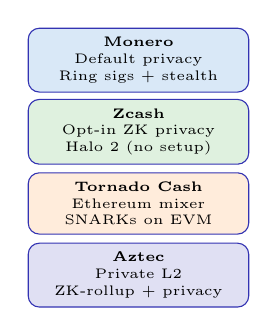
\begin{tikzpicture}[scale=0.7, every node/.style={font=\tiny},
  bx/.style={rounded corners, draw=mlpurple, minimum width=2.8cm, minimum height=0.7cm, align=center}]
\node[bx, fill=mlblue!15] at (0,3.5) {\textbf{Monero}\\Default privacy\\Ring sigs + stealth};
\node[bx, fill=mlgreen!15] at (0,2.2) {\textbf{Zcash}\\Opt-in ZK privacy\\Halo 2 (no setup)};
\node[bx, fill=mlorange!15] at (0,0.9) {\textbf{Tornado Cash}\\Ethereum mixer\\SNARKs on EVM};
\node[bx, fill=mlpurple!15] at (0,-0.4) {\textbf{Aztec}\\Private L2\\ZK-rollup + privacy};
\end{tikzpicture}
\end{center}
\vspace{0.1cm}
\begin{exampleblock}{\footnotesize Next Section}
\footnotesize
$\Rightarrow$ \textbf{ZK Applications:} Rollups, identity, voting, and private DeFi.
\end{exampleblock}
\end{columns}
\bottomnote{Privacy technology evolves rapidly -- new solutions emerge as older ones face regulatory or technical challenges}
\end{frame}

%% ===== SECTION 4: ZK Applications -- Rollups, Identity, Voting, DeFi =====
\section{ZK Applications}

% Frame 37: ZK-Rollup Architecture
\begin{frame}{ZK-Rollups: Architecture Overview}
\begin{center}
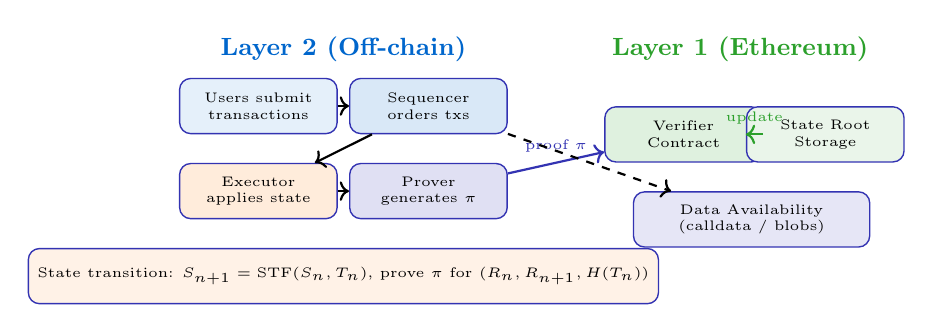
\begin{tikzpicture}[scale=0.72, every node/.style={font=\tiny},
  bx/.style={rounded corners, draw=mlpurple, minimum width=2cm, minimum height=0.7cm, align=center, line width=0.5pt}]
% L2 side
\node[font=\small\bfseries, mlblue] at (-3,5) {Layer 2 (Off-chain)};
\node[bx, fill=mlblue!10] (users) at (-4.5,4) {Users submit\\transactions};
\node[bx, fill=mlblue!15] (seq) at (-1.5,4) {Sequencer\\orders txs};
\node[bx, fill=mlorange!15] (exec) at (-4.5,2.5) {Executor\\applies state};
\node[bx, fill=mlpurple!15] (prover) at (-1.5,2.5) {Prover\\generates $\pi$};
% L1 side
\node[font=\small\bfseries, mlgreen] at (4,5) {Layer 1 (Ethereum)};
\node[bx, fill=mlgreen!15] (verifier) at (3,3.5) {Verifier\\Contract};
\node[bx, fill=mlgreen!10] (state) at (5.5,3.5) {State Root\\Storage};
\node[bx, fill=mllavender!30, minimum width=3cm] (da) at (4.2,2) {Data Availability\\(calldata / blobs)};
% Arrows
\draw[->, thick] (users) -- (seq);
\draw[->, thick] (seq) -- (exec);
\draw[->, thick] (exec) -- (prover);
\draw[->, thick, mlpurple] (prover) -- node[above, font=\tiny]{proof $\pi$} (verifier);
\draw[->, thick, mlgreen] (verifier) -- node[above, font=\tiny]{update} (state);
\draw[->, thick, dashed] (seq) -- (da);
% State transition
\node[bx, fill=mlorange!10, minimum width=8cm] at (-3,1) {State transition: $S_{n+1} = \text{STF}(S_n, T_n)$, prove $\pi$ for $(R_n, R_{n+1}, H(T_n))$};
\end{tikzpicture}
\end{center}
\vspace{0.1cm}
\begin{columns}[T]
\column{0.48\textwidth}
\begin{block}{\footnotesize Why ZK-Rollups?}
\footnotesize
\begin{itemize}
\item \textbf{Scalability}: 1000--2000+ TPS vs Ethereum's $\sim$15 TPS
\item \textbf{Security}: Inherits L1 security via validity proofs
\item \textbf{Finality}: Instant once proof verified on L1
\end{itemize}
\end{block}
\column{0.48\textwidth}
\begin{block}{\footnotesize Data Availability (EIP-4844)}
\footnotesize
\begin{itemize}
\item \textbf{Calldata}: Expensive, permanently stored
\item \textbf{Blobs}: Cheaper, pruned after $\sim$18 days
\item Proto-danksharding reduces L2 costs by 10--100$\times$
\end{itemize}
\end{block}
\end{columns}
\bottomnote{ZK-rollups process transactions off-chain but post validity proofs on-chain -- ``don't trust, verify (efficiently)''}
\end{frame}

% Frame 38: zkEVM Types
\begin{frame}{zkEVM: Types and Tradeoffs}
\footnotesize
\begin{center}
\begin{adjustbox}{max width=\textwidth}
\begin{tabular}{c l l l l}
\toprule
\textbf{Type} & \textbf{Description} & \textbf{Compatibility} & \textbf{Proving Cost} & \textbf{Projects} \\
\midrule
\textbf{1} & Fully Ethereum-equivalent & Exact consensus rules & Very high & Taiko \\
\textbf{2} & EVM-equivalent & Same bytecode, diff state & High & Scroll, Polygon zkEVM \\
\textbf{2.5} & EVM + gas adjustments & Minor gas differences & Moderate--High & -- \\
\textbf{3} & Almost EVM-equivalent & Most opcodes supported & Moderate & -- \\
\textbf{4} & Language-equivalent & Compiles Solidity to custom VM & Lower & zkSync Era \\
\bottomrule
\end{tabular}
\end{adjustbox}
\end{center}
\vspace{0.2cm}
\begin{columns}[T]
\column{0.48\textwidth}
\begin{center}
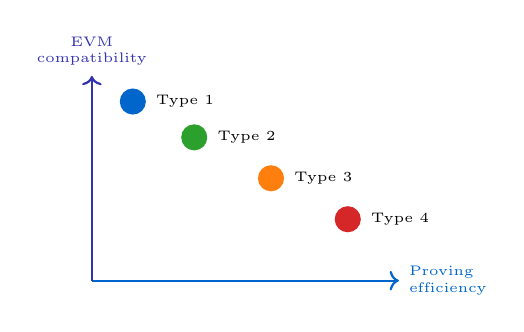
\begin{tikzpicture}[scale=0.65, every node/.style={font=\tiny}]
% Spectrum
\draw[thick, mlblue, ->] (0,0) -- (6,0) node[right, align=left]{Proving\\efficiency};
\draw[thick, mlpurple, ->] (0,0) -- (0,4) node[above, align=center]{EVM\\compatibility};
% Points
\node[circle, fill=mlblue, minimum size=5pt, label=right:{Type 1}] at (0.8,3.5) {};
\node[circle, fill=mlgreen, minimum size=5pt, label=right:{Type 2}] at (2,2.8) {};
\node[circle, fill=mlorange, minimum size=5pt, label=right:{Type 3}] at (3.5,2.0) {};
\node[circle, fill=mlred, minimum size=5pt, label=right:{Type 4}] at (5,1.2) {};
\end{tikzpicture}
\end{center}
\column{0.48\textwidth}
\begin{alertblock}{\footnotesize The Fundamental Tradeoff}
\footnotesize
Higher EVM compatibility $\Rightarrow$ more expensive ZK proving.
\begin{itemize}
\item Type 1: Can verify Ethereum blocks natively
\item Type 4: Fastest proofs but needs recompilation
\item Most projects target Type 2--3 as sweet spot
\end{itemize}
\end{alertblock}
\end{columns}
\bottomnote{Vitalik Buterin's zkEVM taxonomy (2022) provides framework for comparing ZK-rollup approaches to EVM compatibility}
\end{frame}

% Frame 39: ZK-Rollup State Verification
\begin{frame}{ZK-Rollup: State Verification Mathematics}
\begin{columns}[T]
\column{0.50\textwidth}
\begin{block}{\footnotesize State Transition Function}
\footnotesize
\vspace{-0.2cm}
\begin{align*}
S_{n+1} &= \text{STF}(S_n, T_n) \\
R_n &= \text{MerkleRoot}(S_n) \\
R_{n+1} &= \text{MerkleRoot}(S_{n+1})
\end{align*}
where $S_n$ is the state at batch $n$, $T_n$ is the transaction batch, $R_n$ is the state root.
\end{block}
\vspace{0.1cm}
\begin{block}{\footnotesize ZK Proof Statement}
\footnotesize
The prover generates $\pi$ proving:
\begin{enumerate}
\item $\exists\; S_n$ with $\text{Root}(S_n) = R_n$
\item Applying $T_n$ to $S_n$ yields $S_{n+1}$
\item $\text{Root}(S_{n+1}) = R_{n+1}$
\item All transactions in $T_n$ have valid signatures
\item All state updates follow protocol rules
\end{enumerate}
\textbf{Public inputs:} $(R_n, R_{n+1}, H(T_n))$\\
\textbf{Private witness:} $(S_n, T_n, \text{Merkle paths})$
\end{block}
\column{0.48\textwidth}
\begin{block}{\footnotesize L1 Verification}
\footnotesize
The L1 verifier contract checks:
$$\text{Verify}(\text{vk}, \pi, [R_n, R_{n+1}, H(T_n)]) \stackrel{?}{=} \texttt{true}$$
\end{block}
\vspace{0.1cm}
\begin{center}
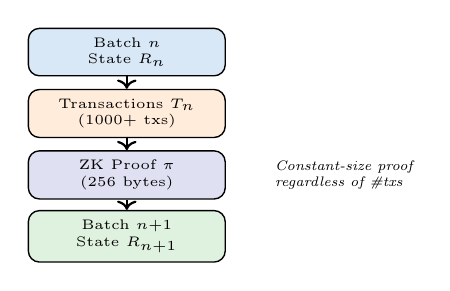
\begin{tikzpicture}[scale=0.65, every node/.style={font=\tiny},
  bx/.style={rounded corners, draw, minimum width=2.5cm, minimum height=0.6cm, align=center, line width=0.5pt}]
% Batch flow
\node[bx, fill=mlblue!15] (b1) at (0,4) {Batch $n$\\State $R_n$};
\node[bx, fill=mlorange!15] (txs) at (0,2.8) {Transactions $T_n$\\(1000+ txs)};
\node[bx, fill=mlpurple!15] (proof) at (0,1.6) {ZK Proof $\pi$\\(256 bytes)};
\node[bx, fill=mlgreen!15] (b2) at (0,0.4) {Batch $n{+}1$\\State $R_{n+1}$};
% Arrows
\draw[->, thick] (b1) -- (txs);
\draw[->, thick] (txs) -- (proof);
\draw[->, thick] (proof) -- (b2);
% Annotation
\node[right=0.5cm, align=left, font=\tiny\itshape] at (proof.east) {Constant-size proof\\regardless of \#txs};
\end{tikzpicture}
\end{center}
\vspace{0.1cm}
\begin{exampleblock}{\footnotesize Compression Ratio}
\footnotesize
1000 transactions $\to$ single 256-byte proof.\\
L1 verification: $\sim$300K gas (constant).
\end{exampleblock}
\end{columns}
\bottomnote{The key insight: verification cost is constant regardless of how many transactions are in the batch}
\end{frame}

% Frame 40: ZK-Rollup Verifier Contract (Solidity Snippet #3)
\begin{frame}[fragile]{ZK-Rollup: L1 Verifier Contract}
\begin{columns}[T]
\column{0.55\textwidth}
\begin{lstlisting}[basicstyle=\fontsize{4.5pt}{5.5pt}\ttfamily]
// SPDX-License-Identifier: MIT
pragma solidity ^0.8.20;

interface IZKVerifier {
    function verifyProof(
        uint[2] calldata a,
        uint[2][2] calldata b,
        uint[2] calldata c,
        uint[3] calldata publicInputs
    ) external view returns (bool);
}

contract ZKRollupVerifier {
    IZKVerifier public immutable zkVerifier;
    bytes32 public stateRoot;
    uint256 public batchNumber;
    address public sequencer;

    event BatchVerified(
        uint256 indexed batch,
        bytes32 oldRoot,
        bytes32 newRoot
    );

    modifier onlySequencer() {
        require(msg.sender == sequencer,
                "Not sequencer");
        _;
    }
\end{lstlisting}
\column{0.43\textwidth}
\begin{lstlisting}[basicstyle=\fontsize{4.5pt}{5.5pt}\ttfamily]
    constructor(
        address _verifier,
        bytes32 _genesisRoot,
        address _sequencer
    ) {
        zkVerifier = IZKVerifier(_verifier);
        stateRoot = _genesisRoot;
        sequencer = _sequencer;
    }

    function verifyBatch(
        uint[2] calldata _a,
        uint[2][2] calldata _b,
        uint[2] calldata _c,
        bytes32 _newRoot,
        bytes32 _txDataHash
    ) external onlySequencer {
        // Public inputs: old root, new root,
        //   transaction data hash
        uint[3] memory inputs = [
            uint256(stateRoot),
            uint256(_newRoot),
            uint256(_txDataHash)
        ];
        require(zkVerifier.verifyProof(
            _a, _b, _c, inputs),
            "Invalid batch proof");
        emit BatchVerified(
            batchNumber, stateRoot, _newRoot);
        stateRoot = _newRoot;
        batchNumber++;
    }
}
\end{lstlisting}
\end{columns}
\bottomnote{Simplified L1 verifier -- production systems include data availability posting, escape hatches, and timelock governance}
\end{frame}

% Frame 41: Zero-Knowledge Identity
\begin{frame}{Zero-Knowledge Identity: Selective Disclosure}
\begin{columns}[T]
\column{0.50\textwidth}
\begin{block}{\footnotesize The Problem}
\footnotesize
Traditional identity verification requires revealing \emph{all} information:
\begin{itemize}
\item Buying alcohol $\to$ show full ID (name, address, DOB)
\item KYC $\to$ upload passport, utility bills, selfies
\item Credit check $\to$ expose full financial history
\end{itemize}
\end{block}
\vspace{0.1cm}
\begin{exampleblock}{\footnotesize ZK Solution: Prove Properties, Not Data}
\footnotesize
With ZK proofs, prove \emph{statements about} your data:
\begin{itemize}
\item ``I am over 18'' (without revealing age)
\item ``I am a citizen of EU'' (without revealing country)
\item ``My credit score $> 700$'' (without revealing score)
\item ``I am not on sanctions list'' (without revealing identity)
\end{itemize}
\end{exampleblock}
\column{0.48\textwidth}
\begin{center}
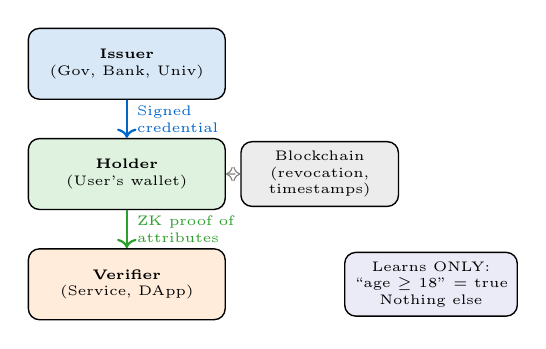
\begin{tikzpicture}[scale=0.7, every node/.style={font=\tiny},
  bx/.style={rounded corners, draw, minimum width=2.5cm, minimum height=0.6cm, align=center, line width=0.5pt}]
% W3C VC flow
\node[bx, fill=mlblue!15, minimum height=0.9cm] (issuer) at (0,4.5) {\textbf{Issuer}\\(Gov, Bank, Univ)};
\node[bx, fill=mlgreen!15, minimum height=0.9cm] (holder) at (0,2.5) {\textbf{Holder}\\(User's wallet)};
\node[bx, fill=mlorange!15, minimum height=0.9cm] (verifier) at (0,0.5) {\textbf{Verifier}\\(Service, DApp)};
% Arrows
\draw[->, thick, mlblue] (issuer) -- node[right, font=\tiny, align=left]{Signed\\credential} (holder);
\draw[->, thick, mlgreen] (holder) -- node[right, font=\tiny, align=left]{ZK proof of\\attributes} (verifier);
% Side note
\node[right=1.5cm, bx, fill=mlpurple!10, minimum width=2cm, font=\tiny] at (verifier.east) {Learns ONLY:\\``age $\geq$ 18'' = true\\Nothing else};
% Blockchain anchor
\node[bx, fill=mlgray!15, minimum width=2cm] (chain) at (3.5,2.5) {Blockchain\\(revocation,\\timestamps)};
\draw[<->, dashed, mlgray] (holder) -- (chain);
\end{tikzpicture}
\end{center}
\end{columns}
\bottomnote{W3C Verifiable Credentials + ZK proofs enable self-sovereign identity where users control their own data}
\end{frame}

% Frame 42: ZK Voting
\begin{frame}{ZK Voting: Private, Verifiable Elections}
\begin{columns}[T]
\column{0.50\textwidth}
\begin{block}{\footnotesize Requirements for Secure Voting}
\footnotesize
\begin{enumerate}
\item \textbf{Eligibility}: Only authorized voters can vote
\item \textbf{Privacy}: No one learns how anyone voted
\item \textbf{Correctness}: Tally accurately reflects all votes
\item \textbf{Coercion resistance}: Cannot prove how you voted to a briber
\end{enumerate}
\end{block}
\vspace{0.1cm}
\begin{exampleblock}{\footnotesize MACI (Minimum Anti-Collusion Infrastructure)}
\footnotesize
\begin{enumerate}
\item Voters encrypt votes with coordinator's public key
\item Coordinator decrypts, tallies, generates ZK proof of correct tally
\item Voters can submit \emph{key change} messages to invalidate earlier votes (anti-coercion)
\item Final tally verified on-chain via ZK proof
\end{enumerate}
\end{exampleblock}
\column{0.48\textwidth}
\begin{center}
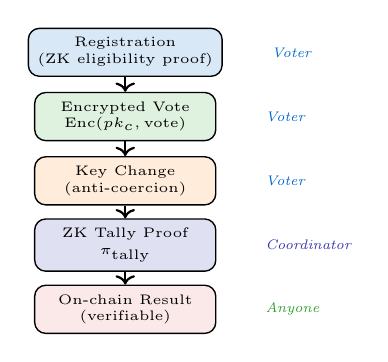
\begin{tikzpicture}[scale=0.68, every node/.style={font=\tiny},
  bx/.style={rounded corners, draw, minimum width=2.3cm, minimum height=0.6cm, align=center, line width=0.5pt}]
% Flow
\node[bx, fill=mlblue!15] (reg) at (0,5) {Registration\\(ZK eligibility proof)};
\node[bx, fill=mlgreen!15] (vote) at (0,3.8) {Encrypted Vote\\$\text{Enc}(pk_c, \text{vote})$};
\node[bx, fill=mlorange!15] (key) at (0,2.6) {Key Change\\(anti-coercion)};
\node[bx, fill=mlpurple!15] (tally) at (0,1.4) {ZK Tally Proof\\$\pi_{\text{tally}}$};
\node[bx, fill=mlred!10] (result) at (0,0.2) {On-chain Result\\(verifiable)};
% Arrows
\draw[->, thick] (reg) -- (vote);
\draw[->, thick] (vote) -- (key);
\draw[->, thick] (key) -- (tally);
\draw[->, thick] (tally) -- (result);
% Side labels
\node[right=0.5cm, font=\tiny\itshape, mlblue] at (reg.east) {Voter};
\node[right=0.5cm, font=\tiny\itshape, mlblue] at (vote.east) {Voter};
\node[right=0.5cm, font=\tiny\itshape, mlblue] at (key.east) {Voter};
\node[right=0.5cm, font=\tiny\itshape, mlpurple] at (tally.east) {Coordinator};
\node[right=0.5cm, font=\tiny\itshape, mlgreen] at (result.east) {Anyone};
\end{tikzpicture}
\end{center}
\end{columns}
\bottomnote{MACI was developed by the Ethereum Foundation and used for Gitcoin grants allocation and DAO governance}
\end{frame}

% Frame 43: Private DeFi
\begin{frame}{Private DeFi: Confidential Finance on-Chain}
\begin{columns}[T]
\column{0.48\textwidth}
\begin{block}{\footnotesize Why Private DeFi?}
\footnotesize
Public DeFi exposes traders to:
\begin{itemize}
\item \textbf{Front-running}: Bots see pending trades in mempool
\item \textbf{MEV extraction}: Miners/validators reorder transactions
\item \textbf{Copy trading}: Competitors mirror your strategy
\item \textbf{Information leakage}: Collateral ratios, positions visible
\end{itemize}
\end{block}
\vspace{0.1cm}
\begin{exampleblock}{\footnotesize ZK Solutions}
\footnotesize
\begin{itemize}
\item \textbf{Dark pools}: Private order books with ZK-proven fair matching
\item \textbf{Confidential balances}: Hidden token amounts
\item \textbf{Private lending}: Hide collateral ratios
\item \textbf{Shielded swaps}: Trade without revealing intent
\end{itemize}
\end{exampleblock}
\column{0.48\textwidth}
\begin{block}{\footnotesize Protocol Examples}
\footnotesize
\begin{tabular}{l l}
\toprule
\textbf{Protocol} & \textbf{Approach} \\
\midrule
Penumbra & Private DEX + staking \\
Aztec & ZK-rollup with privacy \\
Railgun & ERC-20 shielding \\
Renegade & Dark pool matching \\
Panther & Multi-chain privacy \\
\bottomrule
\end{tabular}
\end{block}
\vspace{0.2cm}
\begin{alertblock}{\footnotesize The Trilemma}
\footnotesize
\begin{center}
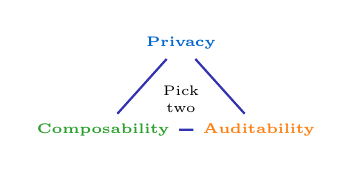
\begin{tikzpicture}[scale=0.55, every node/.style={font=\tiny}]
\node[mlblue, font=\tiny\bfseries] (priv) at (0,2) {Privacy};
\node[mlgreen, font=\tiny\bfseries] (comp) at (-1.8,0) {Composability};
\node[mlorange, font=\tiny\bfseries] (audit) at (1.8,0) {Auditability};
\draw[thick, mlpurple] (priv) -- (comp) -- (audit) -- (priv);
\node[font=\tiny, align=center] at (0,0.7) {Pick\\two};
\end{tikzpicture}
\end{center}
\end{alertblock}
\end{columns}
\bottomnote{MEV (Maximal Extractable Value) cost Ethereum users \$600M+ in 2023 -- private DeFi aims to eliminate this}
\end{frame}

% Frame 44: ZK Machine Learning (zkML)
\begin{frame}{zkML: Verifiable Machine Learning}
\begin{columns}[T]
\column{0.50\textwidth}
\begin{block}{\footnotesize What is zkML?}
\footnotesize
Prove that a machine learning inference was computed correctly \emph{without revealing}:
\begin{itemize}
\item The model weights (proprietary model)
\item The input data (user privacy)
\item Or both (full confidentiality)
\end{itemize}
\end{block}
\vspace{0.1cm}
\footnotesize
\textbf{Applications:}
\begin{itemize}
\item \textbf{Verifiable AI}: Prove an AI model made a specific prediction
\item \textbf{Private inference}: Use a model without revealing your data
\item \textbf{Model marketplace}: Sell predictions without exposing weights
\item \textbf{On-chain AI}: Smart contracts that verify ML outputs
\end{itemize}
\vspace{0.1cm}
\begin{alertblock}{\footnotesize Current Limitations}
\footnotesize
\begin{itemize}
\item Large neural networks: proving is extremely expensive
\item Current: can prove small models (decision trees, small NNs)
\item Research frontier: efficient ZK circuits for matrix multiplication
\end{itemize}
\end{alertblock}
\column{0.48\textwidth}
\begin{center}
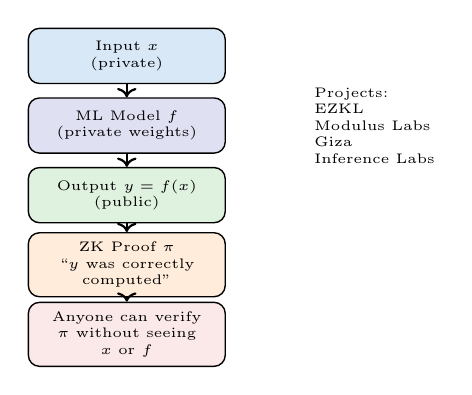
\begin{tikzpicture}[scale=0.68, every node/.style={font=\tiny},
  bx/.style={rounded corners, draw, minimum width=2.5cm, minimum height=0.7cm, align=center, line width=0.5pt}]
% Flow
\node[bx, fill=mlblue!15] (input) at (0,5) {Input $x$\\(private)};
\node[bx, fill=mlpurple!15] (model) at (0,3.7) {ML Model $f$\\(private weights)};
\node[bx, fill=mlgreen!15] (output) at (0,2.4) {Output $y = f(x)$\\(public)};
\node[bx, fill=mlorange!15] (proof) at (0,1.1) {ZK Proof $\pi$\\``$y$ was correctly\\computed''};
\node[bx, fill=mlred!10] (verify) at (0,-0.2) {Anyone can verify\\$\pi$ without seeing\\$x$ or $f$};
\draw[->, thick] (input) -- (model);
\draw[->, thick] (model) -- (output);
\draw[->, thick] (output) -- (proof);
\draw[->, thick] (proof) -- (verify);
% Projects
\node[right=1cm, align=left, font=\tiny] at (model.east) {Projects:\\EZKL\\Modulus Labs\\Giza\\Inference Labs};
\end{tikzpicture}
\end{center}
\end{columns}
\bottomnote{EZKL can generate ZK proofs for ONNX models -- current practical limit is $\sim$10M parameter models}
\end{frame}

% Frame 45: ZK Bridges
\begin{frame}{ZK Bridges: Trustless Cross-Chain Verification}
\begin{columns}[T]
\column{0.50\textwidth}
\begin{block}{\footnotesize The Bridge Problem}
\footnotesize
Cross-chain bridges are the \#1 target for hacks (\$2B+ stolen 2021--2023). Traditional approaches:
\begin{itemize}
\item \textbf{Multisig}: Trust $m$-of-$n$ validators (centralized)
\item \textbf{Optimistic}: Assume valid, challenge period (slow)
\item \textbf{Light client}: Run consensus verification (expensive)
\end{itemize}
\end{block}
\vspace{0.1cm}
\begin{exampleblock}{\footnotesize ZK Bridge Solution}
\footnotesize
\begin{enumerate}
\item Generate ZK proof of Chain A's consensus (block headers, validator signatures)
\item Verify proof on Chain B ($\sim$300K gas)
\item No trusted third parties, no challenge periods
\item Security reduces to ZK proof soundness
\end{enumerate}
\end{exampleblock}
\column{0.48\textwidth}
\begin{center}
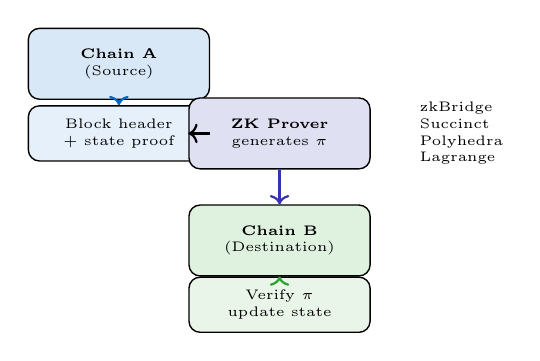
\begin{tikzpicture}[scale=0.68, every node/.style={font=\tiny},
  bx/.style={rounded corners, draw, minimum width=2.3cm, minimum height=0.7cm, align=center, line width=0.5pt}]
% Chain A
\node[bx, fill=mlblue!15, minimum height=0.9cm] (chainA) at (-1,4.5) {\textbf{Chain A}\\(Source)};
\node[bx, fill=mlblue!10] (blockA) at (-1,3.2) {Block header\\+ state proof};
% Prover
\node[bx, fill=mlpurple!15, minimum height=0.9cm] (prover) at (2,3.2) {\textbf{ZK Prover}\\generates $\pi$};
% Chain B
\node[bx, fill=mlgreen!15, minimum height=0.9cm] (chainB) at (2,1.2) {\textbf{Chain B}\\(Destination)};
\node[bx, fill=mlgreen!10] (verify) at (2,0) {Verify $\pi$\\update state};
% Arrows
\draw[->, thick, mlblue] (chainA) -- (blockA);
\draw[->, thick] (blockA) -- (prover);
\draw[->, thick, mlpurple] (prover) -- (chainB);
\draw[->, thick, mlgreen] (chainB) -- (verify);
% Projects
\node[right=0.5cm, align=left, font=\tiny] at (prover.east) {zkBridge\\Succinct\\Polyhedra\\Lagrange};
\end{tikzpicture}
\end{center}
\vspace{0.1cm}
\begin{block}{\footnotesize Security Comparison}
\footnotesize
Multisig: trust validators. ZK: trust math.
\end{block}
\end{columns}
\bottomnote{Ronin Bridge hack (\$625M), Wormhole (\$320M), Nomad (\$190M) -- ZK bridges eliminate the trusted validator attack surface}
\end{frame}

% Frame 46: ZK Coprocessors
\begin{frame}{ZK Coprocessors: Verifiable Off-Chain Computation}
\begin{columns}[T]
\column{0.50\textwidth}
\begin{block}{\footnotesize The Problem}
\footnotesize
Smart contracts are limited:
\begin{itemize}
\item Cannot access historical state cheaply
\item Gas limits constrain computation complexity
\item On-chain data is expensive to process
\item Complex analytics impossible on-chain
\end{itemize}
\end{block}
\vspace{0.1cm}
\begin{exampleblock}{\footnotesize ZK Coprocessor Pattern}
\footnotesize
\begin{enumerate}
\item Query historical blockchain data off-chain
\item Perform complex computation (aggregation, ML, etc.)
\item Generate ZK proof of correct computation
\item Smart contract verifies proof on-chain
\item Result available trustlessly on-chain
\end{enumerate}
\end{exampleblock}
\vspace{0.1cm}
\footnotesize
\textbf{Think of it as:} A trusted computation oracle, where ``trust'' comes from mathematics rather than reputation.
\column{0.48\textwidth}
\begin{center}
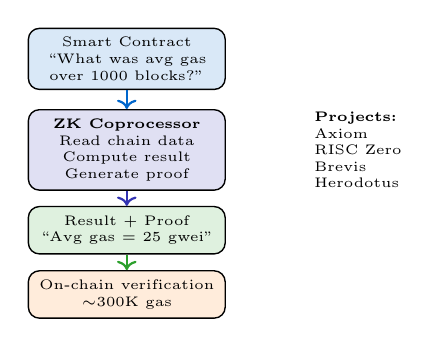
\begin{tikzpicture}[scale=0.68, every node/.style={font=\tiny},
  bx/.style={rounded corners, draw, minimum width=2.5cm, minimum height=0.6cm, align=center, line width=0.5pt}]
% Contract query
\node[bx, fill=mlblue!15] (contract) at (0,5) {Smart Contract\\``What was avg gas\\over 1000 blocks?''};
% Coprocessor
\node[bx, fill=mlpurple!15, minimum height=1cm] (cop) at (0,3.3) {\textbf{ZK Coprocessor}\\Read chain data\\Compute result\\Generate proof};
% Result
\node[bx, fill=mlgreen!15] (result) at (0,1.8) {Result + Proof\\``Avg gas = 25 gwei''};
% Verification
\node[bx, fill=mlorange!15] (verify) at (0,0.6) {On-chain verification\\$\sim$300K gas};
% Arrows
\draw[->, thick, mlblue] (contract) -- (cop);
\draw[->, thick, mlpurple] (cop) -- (result);
\draw[->, thick, mlgreen] (result) -- (verify);
% Projects
\node[right=1cm, align=left, font=\tiny] at (cop.east) {\textbf{Projects:}\\Axiom\\RISC Zero\\Brevis\\Herodotus};
\end{tikzpicture}
\end{center}
\vspace{0.1cm}
\begin{block}{\footnotesize Use Cases}
\footnotesize
Dynamic NFT pricing, on-chain analytics, loyalty rewards based on history, insurance claims verification.
\end{block}
\end{columns}
\bottomnote{ZK coprocessors extend smart contract capabilities without sacrificing trustlessness -- ``SQL for blockchains''}
\end{frame}

% Frame 47: Section 4 Summary
\begin{frame}{Section 4 Summary: ZK Applications}
\begin{columns}[T]
\column{0.48\textwidth}
\begin{center}
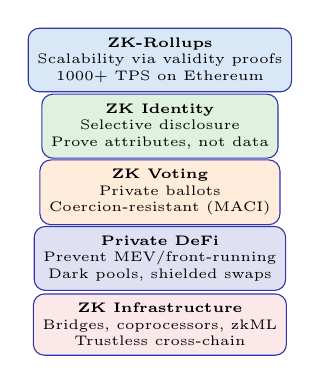
\begin{tikzpicture}[scale=0.7, every node/.style={font=\tiny},
  app/.style={rounded corners, draw=mlpurple, minimum width=3cm, minimum height=0.7cm, align=center}]
\node[app, fill=mlblue!15] at (0,4.2) {\textbf{ZK-Rollups}\\Scalability via validity proofs\\1000+ TPS on Ethereum};
\node[app, fill=mlgreen!15] at (0,3.0) {\textbf{ZK Identity}\\Selective disclosure\\Prove attributes, not data};
\node[app, fill=mlorange!15] at (0,1.8) {\textbf{ZK Voting}\\Private ballots\\Coercion-resistant (MACI)};
\node[app, fill=mlpurple!15] at (0,0.6) {\textbf{Private DeFi}\\Prevent MEV/front-running\\Dark pools, shielded swaps};
\node[app, fill=mlred!10] at (0,-0.6) {\textbf{ZK Infrastructure}\\Bridges, coprocessors, zkML\\Trustless cross-chain};
\end{tikzpicture}
\end{center}
\column{0.48\textwidth}
\begin{block}{\footnotesize Common Pattern}
\footnotesize
All ZK applications follow the same structure:
\begin{enumerate}
\item \textbf{Compute} something privately off-chain
\item \textbf{Prove} correctness with a ZK proof
\item \textbf{Verify} the proof cheaply on-chain
\item \textbf{Trust} mathematics, not intermediaries
\end{enumerate}
\end{block}
\vspace{0.2cm}
\begin{alertblock}{\footnotesize Open Challenges}
\footnotesize
\begin{itemize}
\item Proving costs still high for complex computations
\item Developer tooling immature vs traditional development
\item Regulatory uncertainty around privacy features
\item UX gap: users shouldn't need to understand ZK
\end{itemize}
\end{alertblock}
\vspace{0.1cm}
\begin{exampleblock}{\footnotesize Next Section}
\footnotesize
$\Rightarrow$ \textbf{Advanced Topics:} Hardware acceleration, post-quantum, regulation, and the road ahead.
\end{exampleblock}
\end{columns}
\bottomnote{ZK technology is transitioning from ``interesting cryptography'' to ``critical infrastructure'' for Web3}
\end{frame}

%% ===== SECTION 5: Advanced Topics & Future Directions =====
\section{Advanced Topics \& Future}

% Frame 48: Proving System Frontiers
\begin{frame}{Proving System Frontiers: Next-Generation ZK}
\begin{columns}[T]
\column{0.48\textwidth}
\begin{block}{\footnotesize Lookup-Based Systems}
\footnotesize
\textbf{Lasso \& Jolt} (a16z Research, 2023):
\begin{itemize}
\item Replace arithmetic circuits with \textbf{lookup tables}
\item Prover commits to table entries used
\item Sumcheck protocol verifies consistency
\item 2--10$\times$ faster proving for many operations
\item Jolt: zkVM built entirely on Lasso lookups
\end{itemize}
\end{block}
\vspace{0.1cm}
\begin{block}{\footnotesize Folding Schemes}
\footnotesize
\textbf{Nova} (Kothapalli, Setty, Tzialla 2022):
\begin{itemize}
\item IVC without recursive SNARKs
\item ``Fold'' two instances into one
\item \textbf{HyperNova}: Generalization to CCS (Customizable Constraint Systems)
\item Enables efficient incremental computation
\end{itemize}
\end{block}
\column{0.48\textwidth}
\begin{block}{\footnotesize Binary \& Small Field Systems}
\footnotesize
\textbf{Binius} (Irreducible, 2024):
\begin{itemize}
\item Operates over \textbf{binary fields} $\mathbb{F}_2$
\item Native to how computers actually work
\item No field arithmetic overhead
\item Dramatic speedups for bitwise operations
\end{itemize}
\end{block}
\vspace{0.1cm}
\begin{block}{\footnotesize Circle STARKs}
\footnotesize
\textbf{Stwo} (StarkWare, 2024):
\begin{itemize}
\item STARKs over \textbf{Mersenne prime} $p = 2^{31} - 1$
\item Circle group structure for FFT-like operations
\item 32-bit native arithmetic (CPU-friendly)
\item Expected 10--100$\times$ speedup vs standard STARKs
\end{itemize}
\end{block}
\vspace{0.1cm}
\footnotesize
\textbf{Trend:} Provers are getting faster at roughly 2$\times$/year.
\end{columns}
\bottomnote{The ZK proving landscape is evolving rapidly -- systems that don't exist today may become dominant within 2-3 years}
\end{frame}

% Frame 49: Hardware Acceleration
\begin{frame}{Hardware Acceleration for ZK Proving}
\begin{columns}[T]
\column{0.50\textwidth}
\begin{block}{\footnotesize Why Hardware Matters}
\footnotesize
ZK proving is computationally intensive:
\begin{itemize}
\item Multi-Scalar Multiplication (MSM): $\sum_i s_i \cdot P_i$
\item Number Theoretic Transform (NTT/FFT)
\item Hash computations (Poseidon, Keccak)
\item These operations dominate prover runtime
\end{itemize}
\end{block}
\vspace{0.1cm}
\footnotesize
\begin{center}
\begin{tabular}{l r r}
\toprule
\textbf{Platform} & \textbf{MSM Speed} & \textbf{Cost} \\
\midrule
CPU (single) & 1$\times$ (baseline) & \$ \\
GPU (A100) & 10--50$\times$ & \$\$ \\
FPGA & 20--100$\times$ & \$\$\$ \\
ASIC & 100--1000$\times$ & \$\$\$\$ \\
\bottomrule
\end{tabular}
\end{center}
\column{0.48\textwidth}
\begin{block}{\footnotesize Prover Networks}
\footnotesize
Decentralized proving infrastructure:
\begin{itemize}
\item \textbf{Ingonyama}: GPU-accelerated MSM/NTT
\item \textbf{Cysic}: Custom ZK ASIC development
\item \textbf{Ulvetanna}: FPGA proving clusters
\item \textbf{Gevulot}: Decentralized prover marketplace
\end{itemize}
\end{block}
\vspace{0.1cm}
\begin{alertblock}{\footnotesize Prover Economics}
\footnotesize
Current costs per proof:
\begin{itemize}
\item Simple transfer: \$0.001--0.01
\item zkEVM batch (1000 txs): \$1--10
\item Complex zkML: \$10--100+
\end{itemize}
\textbf{Goal:} Real-time proving on consumer devices (phones, browsers) for client-side ZK.
\end{alertblock}
\end{columns}
\bottomnote{Hardware acceleration is critical for ZK adoption -- the ``prover bottleneck'' is the primary scalability constraint}
\end{frame}

% Frame 50: Post-Quantum ZK
\begin{frame}{Post-Quantum Zero-Knowledge Proofs}
\begin{columns}[T]
\column{0.50\textwidth}
\begin{block}{\footnotesize The Quantum Threat}
\footnotesize
Quantum computers threaten:
\begin{itemize}
\item \textbf{Elliptic curves}: Shor's algorithm breaks ECDLP
\item \textbf{Pairing-based SNARKs}: Groth16, PLONK at risk
\item \textbf{RSA}: Factoring becomes easy
\item \textbf{Not threatened}: Hash functions, symmetric crypto
\end{itemize}
\end{block}
\vspace{0.1cm}
\begin{exampleblock}{\footnotesize Post-Quantum ZK Approaches}
\footnotesize
\begin{itemize}
\item \textbf{STARKs}: Already post-quantum! Based on hash functions and algebraic coding theory (FRI)
\item \textbf{Lattice-based commitments}: Replace Pedersen with lattice schemes (SIS/LWE)
\item \textbf{Hash-based signatures}: Merkle trees + hash chains
\item \textbf{Code-based}: Error-correcting code assumptions
\end{itemize}
\end{exampleblock}
\column{0.48\textwidth}
\footnotesize
\begin{center}
\begin{adjustbox}{max width=0.95\columnwidth}
\begin{tabular}{l c c}
\toprule
\textbf{System} & \textbf{Pre-Q} & \textbf{Post-Q} \\
\midrule
Groth16 & \textcolor{mlgreen}{\checkmark} & \textcolor{mlred}{$\times$} \\
PLONK & \textcolor{mlgreen}{\checkmark} & \textcolor{mlred}{$\times$} \\
Bulletproofs & \textcolor{mlgreen}{\checkmark} & \textcolor{mlred}{$\times$} \\
STARKs & \textcolor{mlgreen}{\checkmark} & \textcolor{mlgreen}{\checkmark} \\
Lattice SNARK & \textcolor{mlgreen}{\checkmark} & \textcolor{mlgreen}{\checkmark} \\
\bottomrule
\end{tabular}
\end{adjustbox}
\end{center}
\vspace{0.2cm}
\begin{alertblock}{\footnotesize NIST Impact}
\footnotesize
NIST PQC standards (2024):
\begin{itemize}
\item ML-KEM (CRYSTALS-Kyber): Key encapsulation
\item ML-DSA (CRYSTALS-Dilithium): Digital signatures
\item SLH-DSA (SPHINCS+): Hash-based signatures
\item ZK community preparing migration paths
\end{itemize}
\end{alertblock}
\end{columns}
\bottomnote{STARKs are naturally post-quantum since they rely only on collision-resistant hash functions, not elliptic curves}
\end{frame}

% Frame 51: Regulation and Ethics
\begin{frame}{Regulatory \& Ethical Dimensions of ZK Privacy}
\begin{columns}[T]
\column{0.48\textwidth}
\begin{alertblock}{\footnotesize The Privacy--Compliance Tension}
\footnotesize
\begin{itemize}
\item \textbf{FATF Travel Rule}: VASPs must share sender/receiver info for transfers $>$ \$1,000
\item \textbf{OFAC Sanctions}: Tornado Cash sanctioned (Aug 2022), developer arrested
\item \textbf{AML/KYC}: Regulators demand identity verification
\item \textbf{EU MiCA}: Limits anonymous crypto transfers
\end{itemize}
\end{alertblock}
\vspace{0.1cm}
\begin{block}{\footnotesize Arguments for Privacy}
\footnotesize
\begin{itemize}
\item Financial privacy is a \textbf{human right} (UN Declaration Art. 12)
\item Businesses need confidentiality (trade secrets, salaries)
\item Protection from surveillance and discrimination
\item Cash transactions are private by default
\end{itemize}
\end{block}
\column{0.48\textwidth}
\begin{exampleblock}{\footnotesize ZK as Middle Ground: Selective Disclosure}
\footnotesize
\textbf{Compliance-friendly privacy:}
\begin{itemize}
\item Prove ``not on sanctions list'' without revealing identity
\item Prove ``KYC'd by approved provider'' without sharing documents
\item Prove ``tax-compliant'' without exposing all transactions
\item \textbf{Privacy Pools} (Buterin et al., 2023): Users prove association with compliant set
\end{itemize}
\end{exampleblock}
\vspace{0.1cm}
\begin{block}{\footnotesize The Spectrum}
\footnotesize
\begin{center}
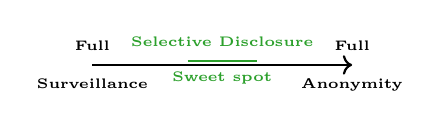
\begin{tikzpicture}[scale=0.55, every node/.style={font=\tiny}]
\draw[thick, ->] (0,0) -- (6,0);
\node[above] at (0,0.1) {\textbf{Full}};
\node[below] at (0,-0.1) {\textbf{Surveillance}};
\node[above] at (6,0.1) {\textbf{Full}};
\node[below] at (6,-0.1) {\textbf{Anonymity}};
\node[above] at (3,0.2) {\textcolor{mlgreen}{\textbf{Selective Disclosure}}};
\draw[mlgreen, thick] (2.2,0.1) -- (3.8,0.1);
\node[mlgreen, font=\tiny\bfseries] at (3,-0.3) {Sweet spot};
\end{tikzpicture}
\end{center}
\end{block}
\end{columns}
\bottomnote{The Tornado Cash case (2022--2024) is a landmark legal battle over whether open-source code constitutes sanctionable ``property''}
\end{frame}

% Frame 52: ZK Developer Ecosystem
\begin{frame}[fragile]{ZK Developer Ecosystem \& Tools}
\begin{columns}[T]
\column{0.48\textwidth}
\footnotesize
\begin{center}
\begin{adjustbox}{max width=\columnwidth}
\begin{tabular}{l l l}
\toprule
\textbf{Tool} & \textbf{Language} & \textbf{Used By} \\
\midrule
Circom & DSL (JS-like) & iden3, Tornado \\
Noir & Rust-like & Aztec \\
Cairo & Rust-like & StarkNet \\
Halo2 & Rust & Zcash, Scroll \\
SP1 & Rust (any code) & RISC Zero \\
Gnark & Go & Consensys \\
\bottomrule
\end{tabular}
\end{adjustbox}
\end{center}
\vspace{0.1cm}
\begin{block}{\footnotesize Circom Example: Hash Preimage}
\footnotesize
\begin{lstlisting}[basicstyle=\fontsize{4.5pt}{5.5pt}\ttfamily,
  morekeywords={pragma,circom,template,signal,input,output,component,main}]
pragma circom 2.1.6;
include "circomlib/poseidon.circom";

template HashPreimage() {
    signal input preimage;
    signal input hash;
    signal output valid;
    // Compute Poseidon hash of preimage
    component hasher = Poseidon(1);
    hasher.inputs[0] <== preimage;
    // Constrain: computed hash == public hash
    hash === hasher.out;
    valid <== 1;
}
component main {public [hash]}
    = HashPreimage();
\end{lstlisting}
\end{block}
\column{0.48\textwidth}
\begin{block}{\footnotesize Development Workflow}
\footnotesize
\begin{enumerate}
\item \textbf{Write circuit} in DSL (Circom, Noir, etc.)
\item \textbf{Compile} to arithmetic circuit (R1CS/PLONK)
\item \textbf{Trusted setup} (if needed) or use universal SRS
\item \textbf{Generate prover/verifier} keys
\item \textbf{Export Solidity verifier} contract
\item \textbf{Deploy} verifier to Ethereum
\item \textbf{Generate proofs} client-side or server-side
\end{enumerate}
\end{block}
\vspace{0.1cm}
\begin{exampleblock}{\footnotesize Emerging Trends}
\footnotesize
\begin{itemize}
\item \textbf{zkVM}: Prove any program (SP1, RISC Zero) -- no circuit writing needed
\item \textbf{Client-side proving}: Generate proofs in browser (WASM)
\item \textbf{Formal verification}: Prove circuits are bug-free
\item \textbf{ZK-as-a-Service}: APIs for proof generation
\end{itemize}
\end{exampleblock}
\end{columns}
\bottomnote{The trend toward zkVMs (prove any Rust/C program) is lowering the barrier to entry for ZK development}
\end{frame}

% Frame 53: The Road Ahead
\begin{frame}{The Road Ahead: ZK as Infrastructure}
\begin{columns}[T]
\column{0.48\textwidth}
\begin{block}{\footnotesize Near-Term (2024--2026)}
\footnotesize
\begin{itemize}
\item zkEVM mainnet maturity (Type 1--2)
\item Client-side proving on mobile devices
\item ZK coprocessors for smart contract analytics
\item Privacy pools for regulatory compliance
\item Proof aggregation across rollups
\end{itemize}
\end{block}
\vspace{0.1cm}
\begin{block}{\footnotesize Medium-Term (2026--2030)}
\footnotesize
\begin{itemize}
\item Universal ZK: prove \emph{any} computation
\item Real-time proving (sub-second for complex circuits)
\item ZK-native identity infrastructure
\item Cross-chain ZK interoperability standard
\item Post-quantum migration for pairing-based systems
\end{itemize}
\end{block}
\column{0.48\textwidth}
\begin{block}{\footnotesize Long-Term Vision}
\footnotesize
\begin{itemize}
\item ``\textbf{Verify, don't trust}'' extends to everything
\item ZK proofs as fundamental internet protocol
\item Private-by-default computation everywhere
\item Provable AI, provable elections, provable finance
\end{itemize}
\end{block}
\vspace{0.1cm}
\begin{center}
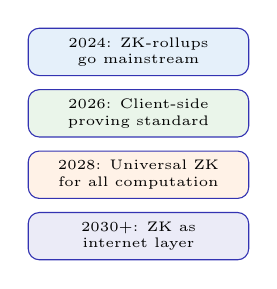
\begin{tikzpicture}[scale=0.65, every node/.style={font=\tiny},
  bx/.style={rounded corners, draw=mlpurple, minimum width=2.8cm, minimum height=0.6cm, align=center}]
\node[bx, fill=mlblue!10] at (0,3.5) {2024: ZK-rollups\\go mainstream};
\node[bx, fill=mlgreen!10] at (0,2.3) {2026: Client-side\\proving standard};
\node[bx, fill=mlorange!10] at (0,1.1) {2028: Universal ZK\\for all computation};
\node[bx, fill=mlpurple!10] at (0,-0.1) {2030+: ZK as\\internet layer};
\end{tikzpicture}
\end{center}
\vspace{0.1cm}
\begin{alertblock}{\footnotesize Open Problems}
\footnotesize
Proof composability, standardization, UX, regulatory clarity, formal verification of circuits.
\end{alertblock}
\end{columns}
\bottomnote{``Zero-knowledge proofs are to computation what public-key cryptography was to communication'' -- paraphrasing Eli Ben-Sasson}
\end{frame}

% Frame 54: Course Summary
\begin{frame}{Course Summary: Privacy \& Zero-Knowledge Proofs}
\begin{columns}[T]
\column{0.48\textwidth}
\begin{block}{\footnotesize ZK Foundations (Section 1)}
\footnotesize
\begin{itemize}
\item Completeness, soundness, zero-knowledge
\item Commitment schemes (Pedersen, KZG)
\item Sigma protocols (Schnorr)
\item Arithmetic circuits $\to$ R1CS $\to$ QAP
\end{itemize}
\end{block}
\vspace{0.1cm}
\begin{block}{\footnotesize Proof Systems (Section 2)}
\footnotesize
\begin{itemize}
\item Groth16: 3-element proofs, trusted setup
\item PLONK: Universal SRS, custom gates
\item STARKs: Transparent, post-quantum, FRI
\item Bulletproofs: No trusted setup, log-size
\end{itemize}
\end{block}
\vspace{0.1cm}
\begin{block}{\footnotesize Privacy Coins (Section 3)}
\footnotesize
\begin{itemize}
\item Monero: Ring sigs + stealth + RingCT
\item Zcash: zk-SNARKs, Halo 2, note model
\item Privacy spectrum: mandatory vs opt-in
\end{itemize}
\end{block}
\column{0.48\textwidth}
\begin{block}{\footnotesize ZK Applications (Section 4)}
\footnotesize
\begin{itemize}
\item ZK-rollups: Scalability via validity proofs
\item zkEVM: Types 1--4 compatibility tradeoff
\item Identity, voting, private DeFi, zkML
\item ZK bridges and coprocessors
\end{itemize}
\end{block}
\vspace{0.1cm}
\begin{block}{\footnotesize Advanced Topics (Section 5)}
\footnotesize
\begin{itemize}
\item Frontier systems: Lasso, HyperNova, Binius
\item Hardware acceleration: GPU/FPGA/ASIC
\item Post-quantum: STARKs already safe
\item Regulation: selective disclosure as middle ground
\end{itemize}
\end{block}
\vspace{0.2cm}
\begin{exampleblock}{\footnotesize Key Takeaway}
\footnotesize
Zero-knowledge proofs transform the trust model of computation: from ``trust the computer'' to ``verify the proof.'' This paradigm shift enables privacy, scalability, and interoperability simultaneously.
\end{exampleblock}
\end{columns}
\bottomnote{ZK proofs are the most important cryptographic primitive since public-key cryptography}
\end{frame}

% Frame 55: Questions & Further Reading
\begin{frame}{Questions \& Further Reading}
\begin{columns}[T]
\column{0.48\textwidth}
\begin{block}{\footnotesize Discussion Prompts}
\footnotesize
\begin{enumerate}
\item Should financial privacy be a \emph{right} or a \emph{privilege}? How does this change with blockchain?
\item Can ZK proofs solve the ``privacy vs compliance'' dilemma, or is it a false dichotomy?
\item Which zkEVM type will dominate, and why?
\item Is Monero's ``privacy by default'' approach superior to Zcash's ``opt-in'' model?
\item What are the implications of zkML for AI governance?
\end{enumerate}
\end{block}
\column{0.48\textwidth}
\begin{block}{\footnotesize Essential Reading}
\footnotesize
\begin{itemize}
\item \textbf{ZKP.science}: Curated ZK proof resources
\item \textbf{Vitalik's blog}: ``An Incomplete Guide to Rollups'', ``The Different Types of ZK-EVMs''
\item \textbf{IACR ePrint}: Latest cryptographic research
\item \textbf{RareSkills ZK Book}: Practical ZK development guide
\item \textbf{0xPARC}: ZK learning resources and grants
\end{itemize}
\end{block}
\vspace{0.1cm}
\begin{exampleblock}{\footnotesize Hands-On Resources}
\footnotesize
\begin{itemize}
\item Circom tutorial: \texttt{docs.circom.io}
\item Noir playground: \texttt{noir-lang.org}
\item zkSNARK interactive demo: \texttt{zkp.science}
\item StarkNet/Cairo: \texttt{starknet.io/learn}
\end{itemize}
\end{exampleblock}
\end{columns}
\bottomnote{``Privacy is not about having something to hide. It is about having something to protect.'' -- Edward Snowden}
\end{frame}

\end{document}
